\documentclass[a4paper,11pt]{article}
\pagestyle{plain}

\usepackage[spanish]{babel}
\usepackage [latin1]{inputenc}
\usepackage{amsthm}
\usepackage{amsmath}
\usepackage{amssymb}
%\usepackage[lined,spanish,boxed,linesnumbered]{algorithm2e}
\usepackage{algorithm}
\usepackage{algpseudocode}
\usepackage[conEntregas]{caratula}
\usepackage[margin=0.75in]{geometry}
\usepackage{listings}
\lstset{breaklines=true}
\usepackage[usenames,dvipsnames]{xcolor}
\definecolor{dkgreen}{rgb}{0,0.6,0}
\definecolor{gray}{rgb}{0.97,0.97,0.97}
\definecolor{mauve}{rgb}{0.58,0,0.82}
\usepackage{tikz}
\usetikzlibrary{arrows}
\usetikzlibrary{babel}
\usepackage{hyperref}
\hypersetup{colorlinks=true,linktocpage}
\newcommand{\theHalgorithm}{\arabic{algorithm}}
\newtheorem{Ejemplo}{Ejemplo}

\begin{document}

\titulo{Trabajo Pr\'actico 3}

\fecha{\today}

\materia{Algoritmos y Estructuras de Datos III}

\integrante{Chapresto, Mat\'ias}{201/12}{matiaschapresto@gmail.com}
\integrante{Dato, Nicol\'as}{676/12}{nico\_dato@hotmail.com}
\integrante{Fattori, Ezequiel}{280/11}{ezequieltori@hotmail.com}
\integrante{Vileri\~no, Silvio}{106/12}{svilerino@gmail.com}

\maketitle

\tableofcontents

%incluye un abstract de lo que trata el trabajo
%\section{Introducci\'on}
%\begin{abstract}
%\end{abstract}



%Incluye el punto 1 del tp
\section{Situaciones de la vida real que pueden ser modeladas con el problema del Camino acotado de costo minimo}
\subsection{Notaci\'on y definiciones iniciales}
Sea un grafo G = (V,E) un grafo simple. Definimos el costo asociado a una funcion $f:E \rightarrow \mathbb{R}_+$ de un camino P = $<v_{1}, \dots, v_{k-1}, v_{k}>$ de la siguiente forma:
\begin{center}
	$costo_f$($P$) = $\sum_{i=1}^{k} f(v_i$)
\end{center}

\subsection{Viaje en ruta: Minimizar la distancia de viaje dada una cantidad fija de dinero}
Sea G = (V, E) un grafo simple, se quiere modelar un mapa de ciudades y rutas entre ellas, para ello definamos V, como el conjunto de nodos donde cada nodo representa una ciudad en el mapa. Asimismo, E ser\'a el conjunto de aristas en donde, sean $v_1,v_2 \in V $ entonces $\exists $ $(v_1,v_2) \in E \Leftrightarrow$ existe una ruta entre las ciudades $v_{1}$ y $v_{2}$. A continuaci\'on definiremos dos funciones sobre el conjunto E de aristas tales que:
\begin{itemize}
	\item $f:E \rightarrow \mathbb{R}_+$: funcion asociada a la distancia entre $v_{src}$ y $v_{dst}$.
	\item $g:E \rightarrow \mathbb{R}_+$: funcion asociada al costo de viajar entre $v_{src}$ y $v_{dst}$.
\end{itemize}
Sea ademas $k \in \mathbb{R}_+$ el dinero del que se dispone para realizar el viaje, el objetivo de esta situacion es, dados $v_1, v_2 \in V$ se quiere llegar de la ciudad $v_{src}$ a la ciudad $v_{dst}$ minimizando la distancia del viaje, pero se debe poder cubrir el costo total del viaje con la cantidad $k$ de dinero disponible.\\
El la siguiente figura se ve un ejemplo de como podria ser un grafo de estas caracteristicas, adem\'as se ve que el camino mas corto en respecto de la funcion distancia $f$, no necesariamente
cumple el requisito de estar dentro de la cota respecto a la funcion de costo $g$ y el dinero disponible $k$. Los pares ordenados en las aristas indican (f: distancia, g: costo).\\

\begin{figure}[H]
	\centering
	\begin{tikzpicture}[shorten >=1pt, auto, node distance=3cm, ultra thick,
   edge_style/.style={draw=black, ultra thick,font=\sffamily\tiny\bfseries}]
	  \node [circle,draw=black,fill=blue!20] (n1) at (1,2) {$v_{src}$};
	  \node [circle,draw=black,fill=blue!20] (n2) at (5,4)  {$v_2$};
	  \node [circle,draw=black,fill=blue!20] (n3) at (3,2)  {$v_3$};
	  \node [circle,draw=black,fill=blue!20] (n4) at (3,0)  {$v_4$};
	  \node [circle,draw=black,fill=blue!20] (n5) at (4,1)  {$v_5$};
	  \node [circle,draw=black,fill=blue!20] (n6) at (7,2)  {$v_6$};
	  \node [circle,draw=black,fill=blue!20] (n7) at (10,2) {$v_{dst}$};

	  \foreach \from/\to/\distance/\cost in {n1/n2/1/5, n1/n3/1/3, n1/n4/2/3, n3/n6/2/4, n5/n6/2/1, n4/n5/1/1, n6/n7/1/1, n2/n7/4/6}
	    \draw [edge_style] (\from) edge node{(\distance, \cost)} (\to);

	\end{tikzpicture}
	\caption{Ejemplo de conexion entre ciudades.} \label{fig:vida_real_1}
\end{figure}
Veamos 3 posibles caminos y analicemos cada uno:
\begin{itemize}
	\item $c_1$ = $<v_{src}, v_2, v_{dst}>$
		\begin{itemize}
			\item dist($c_1$) = 1 + 4 = 5
			\item costo($c_1$) = 5 + 6 = 11
		\end{itemize}
	\item $c_2$ = $<v_{src}, v_3, v_6, v_{dst}>$
		\begin{itemize}
			\item dist($c_2$) = 1 + 2 + 1 = 4
			\item costo($c_2$) = 3 + 4 + 1 = 8
		\end{itemize}
	\item $c_3$ = $<v_{src}, v_4, v_5, v_6, v_{dst}>$
		\begin{itemize}
			\item dist($c_3$) = 2 + 1 + 2 = 5
			\item costo($c_3$) = 3 + 1 + 1 = 5
		\end{itemize}
\end{itemize}
Supongamos que se dispone de K=9 para realizar el viaje, entonces veamos que el camino mas corto seria $c_1$ pero vemos que con esos costos se pasa de K=9, en particular el costo asociado a $c_1$ es 11. Entonces el mejor camino acotando el costo por 9 es $c_2$. Para instancias mas grandes, seguramente no ser\'a facil ver los caminos de esta forma o poder encontrar el \'optimo, ahi es cuando podemos modelar este problema utilizando CACM para lograr el objetivo.

\subsection{Camino mas conveniente segun relieve: Expedicion en la colina}
Otra posible aplicacion para este problema es la siguiente situacion: Se quiere ir de un punto A a otro B en un lugar geografico accidentado, donde existe una zona con un relieve complicado, llamemos C a esta zona, impidiendo cualquier camino directo entre A y B sin pasar por C. La zona accidentada, tiene varias estaciones de reabastecimiento para los viajantes. Procedamos a modelar con grafos la situacion: Sea G = (V, E) un grafo simple, los puntos A y B son dos nodos no adyacentes de G, ambos conectados a una componente conexa C(no necesariamente por una sola arista) (Figura \ref{fig:comp_conexa_ab_c}),luego, como C es conexa y A,B estan ambos conectados con C, existe al menos un camino entre A y B, que pasa por C. Dentro de C, los nodos denotan estaciones de reabastecimiento y si existe una arista entre dos nodos dentro de C, significa que se puede viajar entre dichas estaciones, mas formalmente:\\
Sean $v_1,v_2 \in V $ entonces $\exists $ $(v_1,v_2) \in E$ de peso $ (t, l) \in \mathbb{R_+}^2 \Leftrightarrow$ existe un sendero entre los puntos $v_{1}$ y $v_{2}$ con costo de l litros de nafta que toma t minutos en ser recorrido.
Cada una de las aristas ($v_i, v_j$), tanto entre A,B hacia C o mismas aristas contenidas en C, tienen asociadas dos funciones f,g definidas sobre el conjunto E de aristas del grafo G:
\begin{itemize}
	\item $f:E \rightarrow \mathbb{R}_+$: funcion asociada al tiempo de viaje en minutos entre $v_{i}$ y $v_{j}$.
	\item $g:E \rightarrow \mathbb{R}_+$: funcion asociada al costo de viajar entre $v_{i}$ y $v_{j}$, en cantidad de litros de nafta segun el terreno de dicho sendero.
\end{itemize}

\begin{figure}[H]
	\centering
	\begin{tikzpicture}[shorten >=1pt, auto, node distance=3cm, ultra thick,
   edge_style/.style={draw=black, ultra thick,font=\sffamily\tiny\bfseries}]
	  \node [circle,draw=black,fill=blue!20] (n1) at (1,2) {A};
	  \node [circle,draw=black,fill=orange!20, minimum size=2cm] (n2) at (3,2)  {C};
	  \node [circle,draw=black,fill=blue!20] (n3) at (5,2)  {B};

	  \foreach \from/\to in {n1/n2, n2/n3}
	    \draw (\from) -- (\to);

	\end{tikzpicture}
	\caption{Nodos A,B no adyacentes entre si, conectados a componente conexa C} \label{fig:comp_conexa_ab_c}
\end{figure}

El objetivo es llegar de A a B en la menor cantidad de tiempo, disponiendo de una cantidad fija $K\in \mathbb{R}_+$ de nafta para todo el viaje. Nuevamente este problema puede ser modelado utilizando CACM minimizando la funcion f tal que la funcion g quede acotada por la cantidad K de nafta.

%Incluye los puntos 2.a,2.b,2.c del tp
\section{Algoritmo exacto para la resolucion de CACM}
\subsection{Explicacion detallada del algoritmo propuesto}
\subsection{Complejidad temporal para el peor caso}
\subsection{Nivel de optimalidad de las soluciones}% En grasp no hace falta este inciso por enunciado.
%Describir si es posible instancias de CACM para las cuales el metodo no proporciona una solucion optima.
%Indicar si es posible que tan mala puede ser la solucion obtenida respecto a la solucion optima
%\subsection{Realizar una expermientacion blablabla...todo lo que respecta a testing y benchmarking tiene una subsection para cada punto del tp en la seccion de benchmarking y por ende no hace falta hablar de eso aca}

%Incluye los puntos 3 con todos los algoritmos golosos que se nos ocurran
\section{Heur\'istica Golosa}
\subsection{Explicacion detallada del algoritmo propuesto}

El algoritmo propuesto consta de dos etapas: una etapa de inicializaci\'on y luego el algoritmo goloso propiamente dicho.

\subsubsection{Inicializaci\'on}

Nuestra etapa de inicializaci\'on consta en calcular los caminos m\'inimos en cuanto a costo $w_1$ de todos los nodos hacia el nodo de llegada. Ya que el grafo es simple, las aristas no tienen orientaci\'on definida, por lo cual dados dos nodos $v_1$ y $v_2$, el camino de $v_1$ a $v_2$ es igual al camino de $v_2$ a $v_1$. Esto nos permite ejecutar una \'unica vez el algoritmo de Dikjstra desde el nodo de llegada hasta todos los dem\'as y obtener lo buscado.

\vspace{2mm}

Una vez obtenidos los caminos m\'inimos en cuanto a costo $w_1$, \'estos nos permiten conocer lo siguiente:

\begin{enumerate}
\item Al iniciar el algoritmo, aquellos nodos para los cuales no existe un camino de longitud $w_1 \leq K$ hasta el nodo llegada, los cuales nuestro algoritmo va a ignorar.
\item En medio de la ejecuci\'on del algoritmo, llamando $W_{ac}$ a la acumulac\'on de costos $w_1$ del camino recorrido por el algoritmo hasta ahora, puedo saber si el nodo de la pro\'oxima arista a elegir tiene al menos un camino $c$ hasta el nodo llegada tal que, el costo del camino formado por la uni\'on de $c$ y el recorrido hasta ahora es $\leq K$. En caso de no tenerlo, desde ese nodo no hay un camino v\'alido hasta la llegada, por lo tanto nuestro algoritmo va a descartar esta arista y elegir alguna que tenga al menos un camino posible hasta la llegada. Esto lo podemos conocer, ya que la ejecuci\'on de Dijkstra inicial nos brinda el costo $w_1$ del camino m\'inimo desde el nodo hasta la llegada, por lo tanto  si $W_{ac}$ + $arista$ + $long(minimoCamino)$ $\leq$ $K$ sabemos que existe al menos este camino v\'alido, caso contrario descartamos el nodo.
\end{enumerate}


\begin{center}
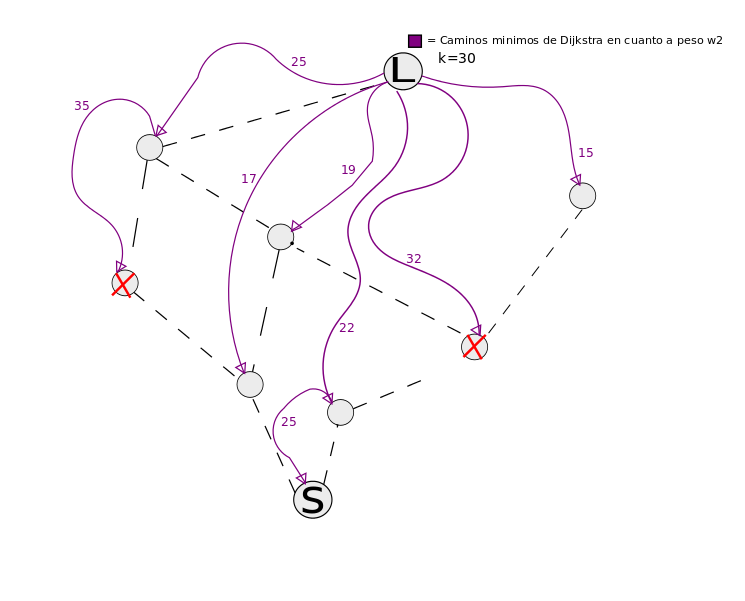
\includegraphics[scale=0.6]{inicializacion.png}
\end{center}
\vspace{2mm}



Esto nos brinda una propiedad invariante: sabemos que en cada iteraci\'on, el costo acumulado del recorrido hecho es necesariamente menor a $K$, y si al menos existe alg\'un un camino de costo menor a $K$ de salida a destino, el algoritmo necesariamente va a poder llegar al nodo de llegada. Deducimos esto al considerar que, o bien no existe ning\'un camino y  el algoritmo termina en la primera iteraci\'on (ya que Dijkstra indica que los caminos m\'inos de costo $K$ de todos los nodos adyacentes a la salida son mayores a $K$, por lo tanto no hay nodo que elegir), o el algoritmo elige una primera arista (por lo tanto existe un camino). 

\vspace{2mm}

Si el algoritmo elige una primera arista, pero luego no logra llegar a destino, significa que en alg\'un punto, desde un nodo $v$ no encontr\'o ninguna arista tal que $W_{ac}$ + $arista$ + $long(minimoCamino)$ $\leq$ $K$. Pero esto no puede ocurrir, ya que en la anterior iteraci\'on, tuvo que elegir necesariamente alguna arista con un extremo en $v$, y el invariante del algortimo nos asegura que desde $v$ existe alg\'un camino v\'alido hasta la llegada, lo cual es absurdo porque el algoritmo se detuvo cuando lleg\'o a $v$. De esta forma concluimos en que, si existe algu\'n camino v\'alido desde la salida hasta la llegada, entonces nuestro algoritmo siempre va a tener como salida un camino v\'alido.

\subsubsection{Algoritmo goloso}

A continuaci\'on se ejecuta el ciclo principal del algoritmo, que genera el CACM usando una heur\'istica golosa. Luego de la ejecuc\'on inicial del algoritmo de Dijkstra, el ciclo principal comienza en el nodo salida y realiza una elecci\'on golosa, la cual es: desde el nodo $v$, descartar las aristas $(v,x)$ incidentes en $v$ tal que $W_{ac}$ + $ss$ + $long(minimoCamino(x))$ $\geq$ $K$. Entre las aristas que quedan, escoger la de menor costo $w_1$.(Aqu\'i se encuentra la desici\'on golosa). El algoritmo itera hasta alcanzar el nodo llegada.

\subsection{Pseudoc\'odigo}


\begin{algorithmic}

\Procedure{$Sol\_Golosa$}{$Grafo\: g, \:vertice\: v_1,\: vertice \: v_2, \: int \: k$}{$\rightarrow lista<eje>\: camino$}

\State $vector<int> \: distancias[g.\#nodos]$
\Comment $ O(n) $
\State $vector<bool> \: visitadas[g.\#aristas]$
\Comment $ O(n) $
\State $ Dijkstra( g, v_2, distancias) $
\Comment $ O() $
\State $lista<eje> \: camino= \emptyset$
\Comment $ O(1) $
\State $ int \: costoCamino = 0 $
\Comment $ O(1) $
\State $ visitadas[v_1] = true $
\Comment $ O(1) $
\State $ vertice \: v_{actual} = v_1 $
\Comment $ O(1) $
\While{ $ actual != v_2 \: || \: incidentes= \emptyset $ }
\Comment $ O(n) $
	\State $ list<eje> \: incidentes = incidentes(v_{actual}, g) $
	\Comment $ O(m) $
	\State $ eje \:	 minimo = primeraNoVisitada(incidentes) $
	\Comment $ O(m) Para\: evitar \:que \:cicle $
	\For {each $(u,v) \in \: incidentes$}
	\Comment $ O(m) $
		\If {$ distancias(v) + costoCamino \leq k \: \&\& \: costo2(u,v) \leq minimo\: \&\& \: visitadas[(u,v)] = false $}
		\Comment $ O(1) $
			\State $ minimo = (u,v) $
			\Comment $ O(1) $
		\EndIf
	\EndFor
	\State $ Agregar(minimo, camino) $
	\Comment $ O(1) $
	\State $ costoCamino \: += costo1(minimo) $
	\Comment $ O(1) $
	\State $ v_{actual} = v $
	\Comment $ O(1) $
\EndWhile
\State $ return \: camino $
\Comment $ O(1) $

\EndProcedure

\end{algorithmic}
\subsection{Complejidad temporal para el peor caso}

La inicializaci\'on ejecuta el algoritmo de Dijkstra, que tiene una complejidad de el nene . El ciclo goloso del algoritmo itera hasta que el v\'ertice actual es igual al v\'ertice de llegada, y recorre como m\'aximo una vez cada v\'ertice (dado el vector visitados), por lo tanto tiene complejidad $O(n)$. Al iniciar el ciclo se ejecuta la funci\'on $incidentes$ que recorre las aristas incidentes en el v\'ertice $actual$, como m\'aximo puede haber $m$ aristas por lo tanto tiene complejidad $O(m)$, y se ejecuta un ciclo $for$ que recorre estas aristas incidentes, por lo tanto tambi\'en $\in$ $O(n)$. Esto nos da una complejidad final de = $ O(el nene)+ O(n)*(O(m)+O(m)) = O(nm)$. 

\subsection{Nivel de optimalidad de las soluciones}

A continuaci\'on vamos a exponer casos en los que la heur\'istica es muy poco eficiente.
\subsubsection{Costos $w_1$ despreciables}

Nuestra heur\'istica se basa fuertemente en asegurarse de que el camino encontrado efectivamente llegue al v\'ertice final, y que el costo $w_1$ acumulado sea menor a $k$, y por esto, uno de sus principales fuerets es el descarte de aristas para los cuales no existen caminos v\'alidos. Pero, si los costos $w_1$ de las aristas son despreciables, es decir, sus valores son muy pequenos (no nulos), de tal forma que el costo de cualquier camino que no repite v\'ertices es siempre menor a $K$, el algoritmo entero se reduce a la elecci\'on golosa de, en cada iteraci\'on, elegir la arista incidente de menor peso y agregarla al camino. Esto puede traer consecuencias como \'esta:

\begin{center}
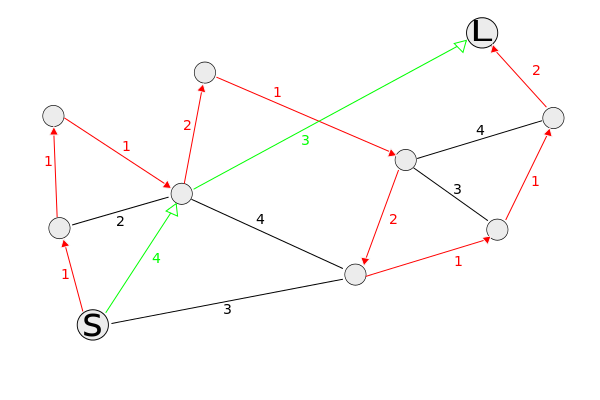
\includegraphics[scale=0.7]{grafoCaminoMasLargo.png}
\end{center}
\vspace{2mm}

La familia de grafos en la cual para todo camino entre dos nodos (que no repita v\'ertices) su costo $w_1$ es siempre menor a $k$. En estos casos el m\'etodo de desici\'on y descarte del algoritmo es inefectivo y s\'olo prima la desici\'on golosa. Vemos en este grafo, que las aristas de menor coste $w_2$ (en color rojo) forman una suceci\'on con un coste final $w_2$ m\'as alto que el camino \'optimo (en verde). Los n\'umeros junto a cada arista son los costos $w_1$, y omitimos los costos $w_2$.

\vspace{2mm}

Hay que destacar que podr\'ia generarse un grafo con una suceci\'on arbitrariamente larga de aristas tal que para cada nodo, la arista de menor peso $w_2$ pertenezca a ella, y que la \'unica arista que incida en el v\'ertice de llegada sea la \'ultima. De esta forma, podemos generarnos grafos de esta familia en los cuales la soluci\'on de nuestra heur\'stica est\'a tan lejos de la \'optima como queramos. De todas formas, el algoritmo nunca se va a quedar ciclando infinitamente, ya que como los costos son no nulos, en alg\'un punto el algoritmo va a descartar la arista que lo lleva de nuevo al ciclo ya que el costo $w_1$ del ciclo + el del camino recorrido ya no va a ser menor o igual a $k$.

\subsubsection{Costos $w_1$ nulos}

En el caso de que las aristas tengan costos $w_1$ nulos, y halla en el grafo un ciclo de pesos $w_2$ m\'inimos el algoritmo no va a terminar.	

%Incluye los puntos 3 con todos los algoritmos de busqueda local que se nos ocurran
\section{Heuristica de busqueda local}

Para encontrar soluciones aproximadas al problema de optimizar una funci\'on $f:S \rightarrow \mathbb{R}$ definida sobre un conjunto $S$ de instancias, la heur\'istica de b\'usqueda local consiste en tomar un elemento $e \in S$ y buscar entre los elementos ``cercanos'' a $e$ uno $e'$ en el cual el valor que toma la funci\'on sea mejor ($f(e') < f(e)$ \'o $f(e') > f(e)$ dependiendo de si se busca m\'inimo a o m\'aximo).
El concepto de cercan\'ia o vecidad se puede definir seg\'un cualquier criterio que se crea conveniente de forma tal que evaluar la vecindad sea barato. Se busca en lo posible que las vecindades de cada punto sean peque\~nas para que se pueda encontrar r\'apidamente un vecino mejor en caso de que exista.
La heur\'istica itera el procedimiento de optimizaci\'on local creando una sucesi\'on de soluciones aproximadas $(X_0, X_1, ... , X_m)$ en $S$ donde el elemento $X_m$ tiene la propiedad de ser un extremo local de la funci\'on $f$ seg\'un el criterio definido de vecindad.

\subsection{Criterios de vecindad}
Para el problema enunciado del TP, el conjunto $S$ es el conjunto de caminos entre el nodo de partida y el de llegada. Debido a que las $w_1$ y $w_2$ son funciones no negativas, el camino acotado de costo m\'inimo estar\'a en $S' \subseteq S$, el subconjunto de todos los caminos simples. Por lo tanto solo se considerar\'a $S'$ como conjunto de instancias.

Establecemos la siguiente notaci\'on: $C = (v_1, ..., v_m)$ ser\'a un camino y $A_c$ el conjunto de aristas que lo conforman. Dos caminos $C = (v_1, ... , v_n)$ y $C' = (v'_1, ... , v'_m)$ en $S'$ son vecinos $C \sim C'$ en su vecindad $N_j$ correspondiente si se cumple su condicion asociada.\\

Definiremos a continuacion varias vecindades:
\begin{enumerate}
    \item $ N_1(C): \exists v \notin C \mid A_{c'} = A_c - \{(v_i,v_{i+1}),(v_{i+1},v_{i+2})\} + \{(v_i,v),(v,v_{i+2})\}$\\
    	Este criterio consiste en reemplazar un nodo intermedio en una tripla, tal que las sumas de los costos $w_2$ de las nuevas aristas sea menor que los costos de las aristas que existian originalmente, teniendo en cuenta tambien, que la mejora no implique que los nuevos costos $w_1$ sobrepasen la cota $K \in \mathbb{R}_{>0}$ establecida en el problema.
    \item $ N_2(C): \exists v \notin C \mid A_{c'} = A_c - \{(v_i,v_{i+1})\} + \{(v_i,v),(v,v_{i+1})\}$\\
    	Este criterio consiste en la inserci\'on de un nodo $v$ adyacente en comun a $v_i$ y $v_{i+1}$ entre ellos, de forma tal que disminuya el costo $w_2$ en el sendero entre $v_i$ $\rightarrow$ $v_{i+1}$ pero que nuevamente no se sobrepase la cota sobre $w_1$ establecida para el problema.
    \item $ N_3(C):  A_{c'} = A_c - \{(v_i,v_{i+1}), (v_{i+1},v_{i+2})\} + \{(v_i,v_{i+2})\}$\\
    	Este criterio consiste en la eliminaci\'on de un nodo intermedio entre una tripla consecutiva de nodos, siendo reemplazado por una arista existente en el grafo que conecte directamente los nodos $v_i$ $\rightarrow$ $v_{i+1}$, de forma tal que la contracci\'on del sendero entre $v_i$ $\rightarrow$ $v_{i+1}$ disminuya el costo $w_2$ pero tampoco sobrepase la cota sobre $w_1$ estipulada en el problema.
    \item $N(C): N_1 \cup N_2 \cup N_3$\\
    	Se trata de la union de todos los criterios anteriores, una exploracion completa de esta vecindad en una iteraci\'on consiste en buscar las mejores modificaciones de las vecindades previas y la aplicacion de la mejor de ellas sobre la solucion actual de dicha iteracion.
\end{enumerate}

\textbf{Nota:} $C = C'$ se considera que son caminos vecinos en todas las vecindades. Adem\'as de los criterios de cada vecindad, debe valer, que el nuevo camino resultante $C'$ sea factible, es decir, respete la cota de $w_1$ de $K$ luego de ser modificado.

\begin{figure}[H]
\centering
\begin{tikzpicture}

\draw[black, solid, very thick] (-1,2) -- (2,1) -- (5,3) -- (6,0) -- (9,1);
\draw[black, dashed, very thick] (2,1) -- (6,0);
\draw[black, dashed, very thick] (2,1) -- (2,-1)  -- (6,0);
\filldraw[fill=green!50!black, draw=black] (2,-1) circle [radius=1mm];
\filldraw[fill=green!50!black, draw=black] (-1,2) circle [radius=1mm];
\filldraw[fill=green!50!black, draw=black] (2,1) circle [radius=1mm];
\filldraw[fill=green!50!black, draw=black] (5,3) circle [radius=1mm];
\filldraw[fill=green!50!black, draw=black] (6,0) circle [radius=1mm];
\filldraw[fill=green!50!black, draw=black] (9,1) circle [radius=1mm];
\node(c) at (3,2) {C};
\node(c') at (3,1) {C'};
\node(c'') at (3,-0.5) {C''};

\end{tikzpicture}
\caption{Tres caminos vecinos entre si.}
\end{figure}

\subsection{Explicacion detallada del algoritmo propuesto}
Sea $s$ una solucion factible, es decir, un camino entre $u,v$ tal que el costo del camino $w_1 \leq K$,
para plantear esta heur\'istica definimos $N(s) = \{ $ conjunto de soluciones vecinas de s$\}$ = $\{$ caminos entre u,v tal que $w_1 \leq K$ y difieren en solo un nodo de $s\}$.\\

Se plantearon 3 posibles enfoques para aplicar busqueda local sobre esta vecindad, a continuacion se explicar\'an cada uno.

\subsubsection{Obtencion de la solucion inicial factible}

Para obtener la solucion inicial factible de nuestra heur\'istica ejecutamos el algoritmo de camino m\'inimo de Dijkstra, entre los nodos u y v, minimizando la funcion $w_1$, acto seguido validamos si $dist(w_1, src, dst) > K$ entonces no existe soluci\'on factible, caso contrario tenemos una soluci\'on factible inicial para comenzar las 
iteraciones de busqueda local.

\subsubsection{Criterio de terminaci\'on}
El criterio de terminacion fue repetir las iteraciones sobre las nuevas soluciones que se iban obteniendo, hasta que no se obtiene mejora.
Pueden aplicarse las iteraciones con exploraciones sobre las vecindades $N_1$, $N_2$, $N_3$ por separado o bien combinarse en $N$ como mencionamos anteriormente. Esto se selecciona mediante un parametro en el metodo main del codigo de la busqueda local.

\subsubsection{Pseudocodigo}

A continuaci\'on el pseudoc\'odigo de la b\'usqueda local.
\begin{algorithmic}

 \Procedure{$Bq\_Local$}{$Grafo\: g, \:vertice\: v_1,\: vertice \: v_2, \: int \: k, tipo\_busqueda$}{$\rightarrow lista<eje>\: camino$}

 \State $lista<eje> \: camino\: =\: dijkstra(g, \:v_1,\: v_2, \:costoW1)$
 \If{camino.costoW1 $>$ K}
 \State No existe solucion.
 \EndIf
 \State  $bool\: valor\_mejora\: = \:\infty$

 \While{$valor\_mejora > 0$}

  \State $switch(tipo\_busqueda)$
	\State$\: \: \: 	case\: subdividirPares$
		\State$\: \: \: \: \: 	\:valor\_mejora\: = \: bqLocalEntrePares(g,camino)$
	\State$	\: \: \: case\: contraerTriplas$		
		\State$\: \: \: \: \: 	\:valor\_mejora\: = \: bqLocalContraerTriplas(g,camino)$
	\State$	\: \: \: case \:mejorarTriplas:		$
		\State$\: \: \: \: \: 	\:valor\_mejora\: = \: bqlocalEntreTriplasReemplazando(g,camino)$
	\State$	\: \: \: case \:combinarVecindades:		$
		\State$\: \: \: \: \: 	\:valor\_mejora\_1\: = \: estimar\_bqLocalEntrePares(g,camino)$
		\State$\: \: \: \: \: 	\:valor\_mejora\_2\: = \: estimar\_bqLocalContraerTriplas(g,camino)$
		\State$\: \: \: \: \: 	\:valor\_mejora\_3\: = \: estimar\_bqlocalEntreTriplasReemplazando(g,camino)$
		\State$\: \: \: \: \: 	\:valor\_mejora\: = \: Aplicar$ $la$ $mejor$ $de$ $las$ $3$ $vecindades$ $exploradas$ $o$ $setear$ $valor\_mejora$ $en$ $0$ $indicando$ $que$ $no$ $se$ $pudo$ $mejorar$ $mas$.


\EndWhile

 \State $return \:camino$

 \EndProcedure

\end{algorithmic}

A continuac\'ion se explicar\'an las vecindades definidas al comienzo de esta secci\'on.

\subsubsection{Reemplazar un nodo intermedio en una 3-upla consecutiva de nodos del camino}
Si el camino tiene longuitud 2, es decir hay una arista directa entre $u,v$ , no hay nada que hacer en este caso, caso contrario, sea $S = \{u,...,v_l, v_{l+1}, v_{l+2}, v_{l+3} ..., v\}$ la solucion actual. Lo que hace en este caso es iterar sobre todas las 3-uplas consecutivas del camino, en este ejemplo sea $(vl, v_{l+1}, v_{l+2})$ una 3-upla, $(v_{l+1}, v_{l+2}, v_{l+3})$ la siguiente a iterar, etc...\\ \\
Para cada 3-upla iterada se revisan los vecinos en comun entre los extremos de la 3-upla buscando una mejor conexi\'on entre extremos reemplazando el nodo intermedio, es decir, se busca una nueva conexion entre los extremos tal que, si el nuevo nodo intermedio es $v_t$, vale que:
\begin{itemize}
	\item Mejore la conexion de la 3-upla respecto a $w_2$, $w_2(vl, v_{t}) + w_2(vt, v_{l+2}) < w_2(vl, v_{l+1}) + w_2(v_{l+1}, v_{l+2})$
	\item Este cambio, reflejado en la nueva solucion candidata S', no sobrepase la cota K establecida sobre $w_1$, es decir, sea factible.
\end{itemize}


Una iteracion consiste en recorrer todas las 3-uplas del camino obteniendo de los vecinos en com\'un de los extremos de cada 3-upla, si es posible, la mejor forma de mejorar esta conexion, ademas recordando la mejor 3-upla para aplicar la mejora a lo largo de la iteraci\'on, tal que el camino resultante de aplicar esta mejora sea el minimo sobre $w_2$ en la vecindad $N_1(s)$. Mas formalmente, se busca una solucion vecina del camino S, tal que siendo $w_1(P), w_2(P)$ los costos sobre $w_1$ y $w_2$ respectivamente de una solucion, y $S' = S \setminus \{(v_k, v_{k+1}); (v_{k+1}, v_{k+2})\} \cup \{(v_k, v_t);(v_t, v_{k+2})\}$ la nueva solucion obtenida, entonces valga que:
\begin{itemize}
	\item Sea factible, pertenezca a $N_1(S)$, $ w_1(S') \leq K$
	\item Sea minima respecto de $w_2$ en la vecindad $N(S)$, $w_2(S') \leq w_2(T)$ $ \forall$ $ T \in N(S) $
\end{itemize}

\subsubsection{Insertar un nodo intermedio en un par consecutivo de nodos del camino}
Este enfoque es basicamente igual al anterior, solo que en lugar de iterar sobre 3-uplas reemplazando el nodo intermedio, se itera sobre pares consecutivos de nodos de la solucion S $(v_k, v_{k+1})$ buscando si existe, un vecino en comun entre los extremos tal que el sendero $(v_k, v_t, v_{k+1})$ tenga costo menor(de forma minima entre los vecinos) sobre $w_2$ que la arista directa y que reflejado en la solucion candidata S' que surge de aplicar este cambio, siga siengo factible($w_2(S') \leq K$). La iteracion de sigue siendo sobre toda la vecindad $N_2(S)$ y quedandose con el mejor $S' \in N_2(S)$ posible.


\subsubsection{Contracci\'on de 3-uplas}

Similar a los casos anteriores, itera sobre las 3-uplas de nodos del camino, intentando eliminar el nodo intermedio y buscar una arista que conecte directamente los nodos de los extremos. Sean los 3 nodos $v_1$, $v_2$ y $v_3$, y el subcamino de aristas formado por ellos $[ (v_1, v_2), (v_2, v_3)]$, se encontrar la arista $(v_1, v_3)$, tal que:

\begin{itemize}
	\item $costoW2((v_1, v_3)) \leq costoW2((v_1, v_2)) + costoW2((v_2, v_3))$
	\item Que el camino, eliminando el nodo $v_2$ y las aristass $(v_1, v_2), (v_2, v_3)$ y conectando los nodos $v_1$ y $v_3$ mediante la arista directa $(v_1, v_3)$ siga sin sobrepasar la cota K establecida sobre $w_1$, es decir, sea factible.
\end{itemize}

\subsection{Nivel de optimalidad de las soluciones}
\subsubsection{Familias de grafos malas para esta heur\'istica}

La heur\'istica va a fallar en todos los casos en los cuales no se pueda mejorar un par o tripla de nodos agregando, quitando o reemplazando de a un nodo, por ejemplo, casos en los que la mejora entre dos nodos sea un subcamino de longitud mayor a 2, o casos en los que el camino \'optimo no tiene ning\'in tipo de conexi\'on con el camino m\'inimo seg\'un $w_1$. Podria intentar arreglarse el problema generalizando la idea de contraer triplas a contraer subcaminos consecutivos de mayor longuitud con alguna variaci\'on de BFS pero podr\'ia incrementarse mucho el cardinal de las vecindades, siendo esto un problema para la exploraci\'on de las mismas.

En el proximo ejemplo. Mostraremos un grafo en el cual la heur\'istica no devuelve la soluci\'on \'optima.

\begin{figure}[H]
	\centering
	\begin{tikzpicture}[shorten >=1pt, auto, node distance=3cm, ultra thick,
   edge_style/.style={draw=black, ultra thick,font=\sffamily\tiny\bfseries}]
	\node [circle,draw=black,fill=blue!20] (n1) at (1,2)  {$v_1$};
	\node [circle,draw=black,fill=blue!20] (n6) at (3,4)  {$v_6$};
	\node [circle,draw=black,fill=blue!20] (n2) at (3,0)  {$v_2$};
	\node [circle,draw=black,fill=blue!20] (n7) at (4,2)  {$v_7$};
	\node [circle,draw=black,fill=blue!20] (n3) at (5,-1)  {$v_3$};
	\node [circle,draw=black,fill=blue!20] (n4) at (7,0)  {$v_4$};
	\node [circle,draw=black,fill=blue!20] (n8) at (7,2)  {$v_8$};
	\node [circle,draw=black,fill=blue!20] (n5) at (9,2)  {$v_5$};

	\foreach \from/\to/\distance/\cost in {
		n1/n6/3/1,
		n1/n7/2/7,
		n1/n2/3/5,
		n6/n7/4/2,
		n2/n7/4/1,
		n6/n5/8/1,
		n2/n3/4/1,
		n3/n4/1/2,
		n4/n5/1/3,
		n7/n8/1/7,
		n8/n5/1/3,
		n7/n3/1/1,
		n3/n8/1/3
		}
	  \draw [edge_style] (\from) edge node{(\distance, \cost)} (\to);
	
	\path (n1) edge [bend left=83, draw=red!50] node{(10, 1)} (n5);

	\end{tikzpicture}
	\caption{Ejemplo grafo malo para la heur\'istica.} \label{fig:vida_real_1}
\end{figure}

Para esta entrada, la soluci\'on inicial factible que nos brinda el algoritmo de dijkstra comienza siendo:\\
\textbf{Nota: } Los pesos entre corchetes representan a $w_1$ y $w_2$ respectivamente.
\begin{lstlisting}[frame=single]
	Camino inicial: (1)----[2, 7]---->(7)----[1, 7]---->(8)----[1, 3]---->(5)
\end{lstlisting}

La cual no tiene ninguna relaci\'on con la soluci\'on \'optima. La b\'usqueda local finaliza devolviendo un camino:
\begin{lstlisting}[frame=single]
	(1)----[3, 1]---->(6)----[4, 2]---->(7)----[1, 1]---->(3)----[1, 2]---->(4)----[1, 3]---->(5)	
\end{lstlisting}

Veamos que no es el camino \'optimo:
Salida del algoritmo de soluci\'on exacta
\begin{lstlisting}[frame=single]
	10 1 2 1 5, es decir. La arista directa entre (1) y (5) con un peso w1: 10 y peso w2: 1
\end{lstlisting}

Otro ejemplo, en el cual el camino que devuelve el dijkstra inicial, y el camino \'optimo son disjuntos en nodos, por lo cual no hay ninguna mejora para hacer, y con lo cual vemos que la soluci\'on de la heur\'istica puede alejarse de la \'optima arbitrariamente.

\begin{figure}[H]
	\centering
	\begin{tikzpicture}[shorten >=1pt, auto, node distance=3cm, ultra thick,
   edge_style/.style={draw=black, ultra thick,font=\sffamily\tiny\bfseries}]
	\node [circle,draw=black,fill=blue!20] (n1) at (1,2)  {$v_1$};
	\node [circle,draw=black,fill=blue!20] (n2) at (3,4)  {$v_2$};
	\node [circle,draw=black,fill=blue!20] (n3) at (6,4)  {$v_3$};
	\node [circle,draw=black,fill=blue!20] (n4) at (3,0)  {$v_4$};
	\node [circle,draw=black,fill=blue!20] (n5) at (6,0)  {$v_5$};
	\node [circle,draw=black,fill=blue!20] (n6) at (8,2)  {$v_6$};
	

	\foreach \from/\to/\distance/\cost in {
		n1/n2/1/3,
		n2/n3/1/2,
		n3/n6/1/3,
		n1/n4/2/1,
		n4/n5/3/1,
		n5/n6/1/3
		}
	  \draw [edge_style] (\from) edge node{(\distance, \cost)} (\to);
	
	

	\end{tikzpicture}
	\caption{Ejemplo grafo malo para la heur\'istica.} \label{fig:vida_real_1}
\end{figure}

\begin{lstlisting}[frame=single]
Camino inicial: (1)----[1, 3]---->(2)----[1, 2]---->(3)----[1, 3]---->(6)
\end{lstlisting}

Soluci\'on final de la heur\'istica:


\begin{lstlisting}[frame=single]
(1)----[1, 3]---->(2)----[1, 2]---->(3)----[1, 3]---->(6)
\end{lstlisting}

Veamos que no es el \'optimo. Soluci\'on del algoritmo exacto:

\begin{lstlisting}[frame=single]
6.000000 5.000000 4 1 4 5 6
\end{lstlisting}

Donde vemos que el camino \'optimo es el 1,4,5,6. Esto se da por la poca densidad del grafo, y en particular, por ser disjuntos los caminos de salida a llegada, la b\'usqueda local no encuentra mejora para realizar y se queda con la soluci\'on que brinda el dijkstra inicial.

Es f\'acil notar que el hecho de agregarle aristas al grafo, posibilita a la b\'usqueda a comenzar a realizar mejoras, por lo tanto el algoritmo funciona mejor para grafos con una mayor densidad de aristas. Vamos a realizar pruebas sobre esto en la secci\'on de experimentaci\'on.

\subsection{Complejidad}
Para la explorac\'ion de las vecindades $N_1$ y $N_2$ se recorren las duplas/triplas consecutivas de nodos, segun corresponda, lo cual toma $O(n)$, y por cada una de las triplas, se obtienen los vecinos en comun de los nodos extremos, esto cuesta $O(n)$, sin embargo, fue mejorada la constante debido a un preprocesamiento mencionado debajo. Luego la complejidad temporal de explorar sucesivamente las vecindades mencionadas es $k*O(n^2)$, donde k es la cantidad de iteraciones necesarias hasta finalizar la b\'usqueda local.\\
Para la vecindad $N_3$ se recorren todas las triplas consecutivas, nuevamente con un costo temporal de \'orden lineal. Para cada tripla, se verifica en tiempo constante por matriz de adyacencia que exista una arista directa entre los extremos y se validan las restricciones de factibilidad y mejora de $w_1$ y $w_2$ respectivamente. Luego, el costo temporal de exploracion sucesiva se la vecindad es $k*O(n)$, donde k es la cantidad de iteraciones que fueron realizadas hasta finalizar la b\'usqueda local.\\

\textbf{Complejidad exploracion combinada:} En este caso la exploraci\'on completa de la vecindad $N$ consiste en una exploracion consecutiva de las vecindades $N_1, N_2, N_3$, con lo cual la complejidad de explorar toda la vecindad, es la suma de las complejidades de las vecindades que la componen, es decir $O(n) + O(n^2) + O(n^2) $ = $ O(n^2)$. Luego de la exploracion, en tiempo constante se obtiene la mejora factible que mas impacte en la minimizacion de $w_2$ y se la aplica en tiempo constante dado que el camino esta implementado con listas enlazadas, y poseemos el iterador al punto del camino a modificar, ya sea insertando o eliminando nodos. El costo temporal total de la b\'usqueda local combinada es $k*O(n^2)$ donde k es la cantidad de iteraciones que fueron necesarias hasta obtener el extremo local.\\

\textbf{Nota:} Se acotan por $O(n)$ los recorridos de triplas y duplas consecutivas, porque se mantiene siempre un camino \texttt{simple} y a lo sumo contiene a todos los nodos del grafo, es decir que el camino tiene longuitud n como m\'aximo. 

\subsection{Taboo list}
  Definimos una taboo list como una lista en la cual se encuentran los nodos que pertenecen al camino soluci\'on actual, de forma de evitar que la b\'usqueda local intente mejorar las conexiones utilizano nodos que ya pertenecen al camino.Esto es indispesable para evitar la generacion de ciclos en el caso de agregar un nodo al subdividir una arista o reemplazar un nodo
intermedio entre otros dos. Si se mantienen disjuntos disjuntos el conjunto de nodos del camino actual y los nodos restantes del grafo, cualquier eleccion que hagamos no generar\''a ciclos.

\vspace{2mm}

La taboo list est\'a implementada como un vector de bool que forma parte de los atributos de un camino del grafo, de forma de poder consultar la pertenencia de un nodo al camino en tiempo constante.

\vspace{2mm}

	Otra opcion considerada fue no restringir la b\'usqueda de nuevos nodos, pero luego deber\'ia realizarse una poda de ciclos del camino. En la muchos de los casos esto realizari\'ia una mejora importante del camino, pero esto aumenta la complejidad de la heur\'istica y deja de ser b\'usqueda local, dado que la soluci\'on que surja de la poda en muchos casos no va a estar en la vecindad del camino.
 
\subsection{Prec\'omputo de vecinos en comun}
Para agilizar la b\'usqueda de vecinos en comun entre 2 nodos para la exploracion de las vecindades y aprovechando que el grafo es estatico, es decir, no se agregan o quitan aristas luego de ser leido de la entrada, se precomputa, para cada par de nodos $v_i,v_j$ una lista con los nodos adyacentes en comun. Luego para obtener los vecinos en comun en los diversos algoritmos implementados, solo basta con obtener esta informaci\'on precomputada.

\subsection{Experimentacion: Mediciones de Performance}
En esta secci\'on se mostrar\'an resultados de complejidad temporal emp\'irica acerca del costo promedio de una iteracion de busqueda local, veremos que tal como analizamos en la secci\'on anterior de complejidad, dicho costo esta situacion en el orden cuadratico $O(n^2)$.
Para tener una mejor idea del comportamiento del algoritmo, realizamos pruebas sobre grafos aleatorios de distintos tama\~nos(en cantidad de nodos), y por cada cantidad $n$ de nodos, variamos las densidades de aristas dentro de cierto rango alrededor de una funcion de $n$, las densidades elegidas fueron:
\begin{itemize}
	\item m = $a*n + b$. Es decir una cantidad lineal de aristas en base a los nodos. $a \in \mathbb{N}_{>1}$
	\item m = $\frac{n*(n-1)}{2}$. Es decir grafos cercanos o iguales a cliques de n nodos.
\end{itemize}


\textbf{Nota: } Como mencionamos anteriormente, las funciones son variadas en un rango, es decir, por ejemplo, para el caso de cliques, los grafos generados tienen entre $\frac{n*(n-1)}{5}$ y $\frac{n*(n-1)}{2}$ aristas para aleatorizar mas la generacion de grafos densos.\\

\textbf{Nota: } Los graficos que contienen puntos rojos y una curva verde, indican, para cada valor del eje X(cantidad de nodos), los puntos rojos son los tiempos de ejecucion para los diferentes valores de aristas en el rango de la familia, asimismo, la curva verde indica el promedio de estos puntos para cada X. \\
\textbf{Nota: }Para verificar que se trata de una curva cuadratica dividimos las funciones por $n^1$, $n^2$, $n^3$, $n^4$ y como en los trabajos practicos anteriores concluimos de que curva se trata.\\

A continuacion presentamos los resultados de estos experimentos:\\
\subsubsection{Rendimiento para grafos con densidad lineal de aristas}
\begin{itemize}
	\item cant nodos min = $200$
	\item cant nodos max = $2000$
	\item peso maximo w1 = $200$
	\item peso maximo w2 = $200$
	\item step nodos = $200$
	\item step aristas = $2500$
	\item aristas minimas = $n-1$
	\item aristas maximas = $10*n$
\end{itemize}								

\begin{center}
	\textbf{Tiempo de ejecuci\'on en microsegundos para esta familia}\\
	\textbf{$y = f(x)$}\\
	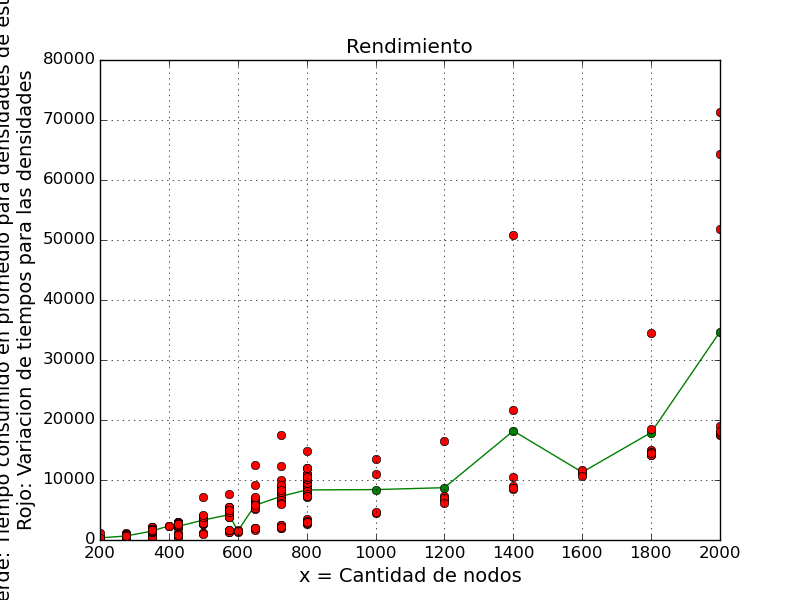
\includegraphics[scale=0.7]{experimentos/bqlocal/rendimiento_aristas_lineales/complexity_variation.png}
\end{center}

\begin{center}
	\textbf{$y = f(x)/x$}\\
	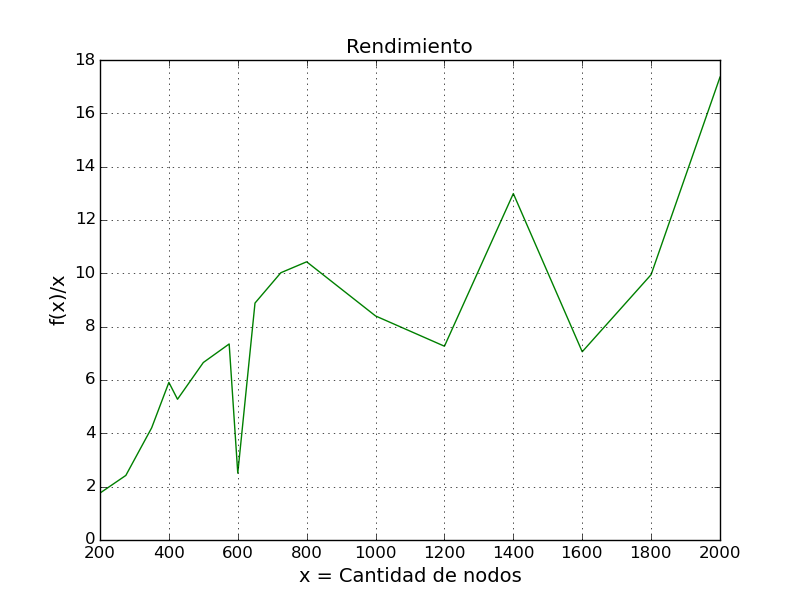
\includegraphics[scale=0.7]{experimentos/bqlocal/rendimiento_aristas_lineales/complexity_med_over_n.png}
\end{center}

\begin{center}
	\textbf{$y = f(x)/x^2$}\\
	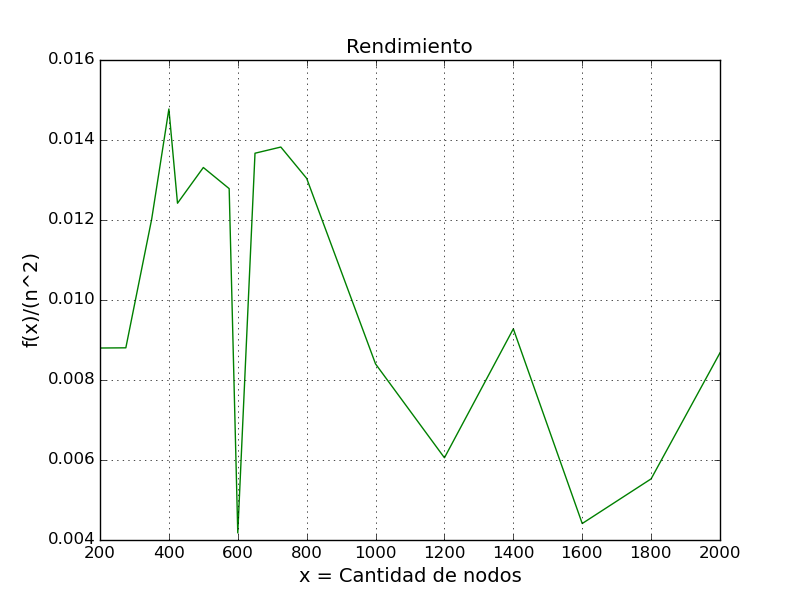
\includegraphics[scale=0.7]{experimentos/bqlocal/rendimiento_aristas_lineales/complexity_med_over_n_square.png}
\end{center}

\begin{center}
	\textbf{$y = f(x)/x^3$}\\
	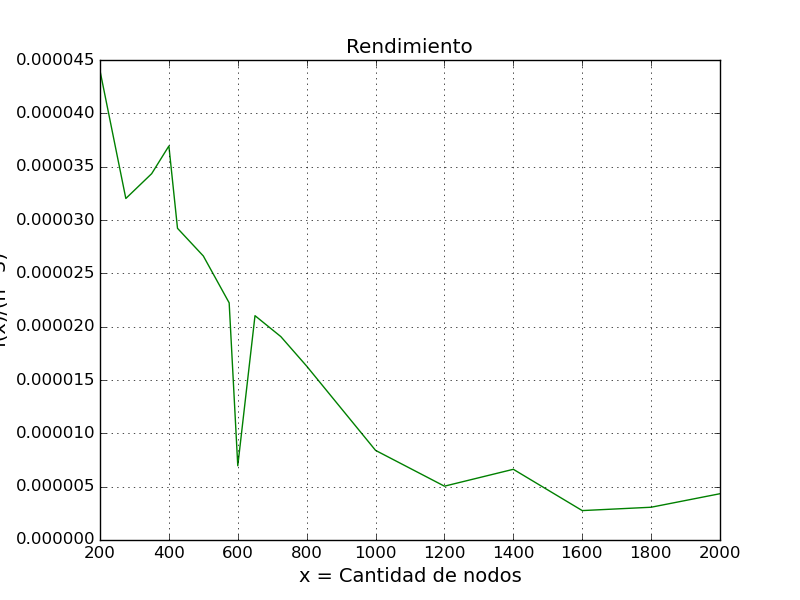
\includegraphics[scale=0.7]{experimentos/bqlocal/rendimiento_aristas_lineales/complexity_med_over_n_cube.png}
\end{center}

\begin{center}
	\textbf{$y = f(x)/x^4$}\\
	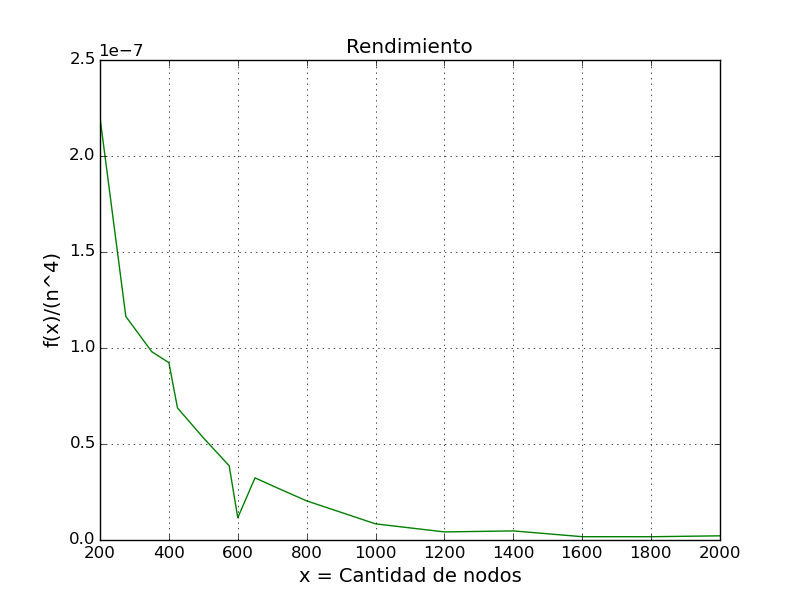
\includegraphics[scale=0.7]{experimentos/bqlocal/rendimiento_aristas_lineales/complexity_med_over_n_fourth.png}
\end{center}

\subsubsection{Rendimiento para grafos con densidad cuadratica de aristas}
\begin{itemize}
	\item cant nodos min = $100$
	\item cant nodos max = $2000$
	\item peso maximo w1 = $200$
	\item peso maximo w2 = $200$
	\item step nodos = $200$
	\item step aristas = $2500$
	\item aristas minimas = $\frac{n*(n-1)}{17}$
	\item aristas maximas = $\frac{n*(n-1)}{14}$
\end{itemize}								

\begin{center}
	\textbf{Tiempo de ejecuci\'on en microsegundos para esta familia}\\
	\textbf{$y = f(x)$}\\
	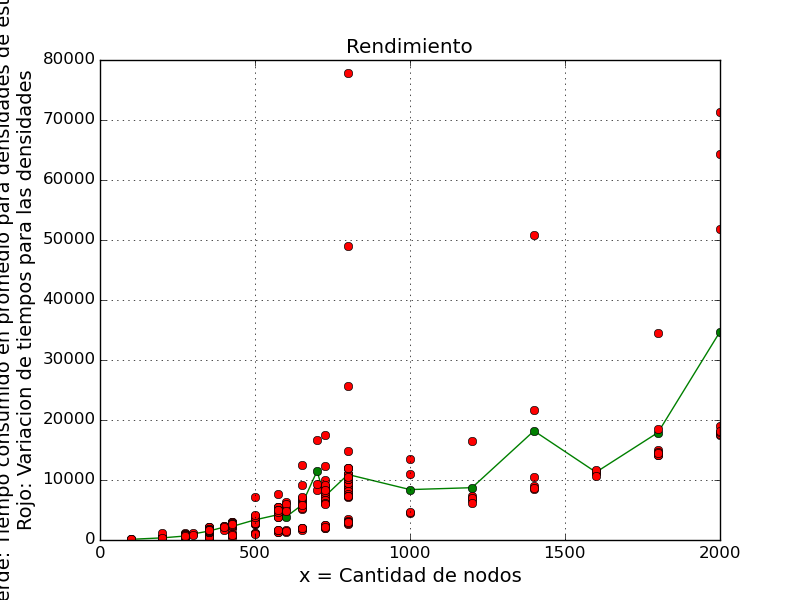
\includegraphics[scale=0.7]{experimentos/bqlocal/rendimiento_aristas_cuadraticas_3/complexity_variation.png}
\end{center}

\begin{center}
	\textbf{$y = f(x)/x$}\\
	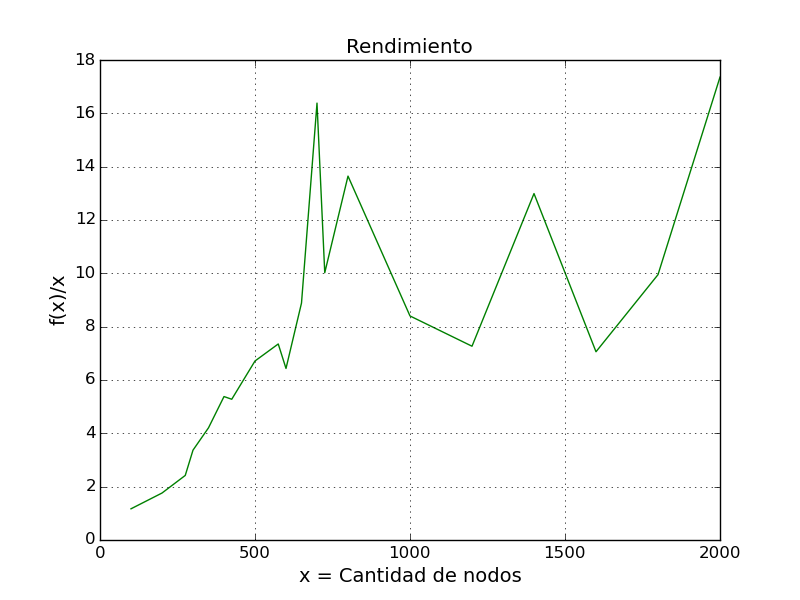
\includegraphics[scale=0.7]{experimentos/bqlocal/rendimiento_aristas_cuadraticas_3/complexity_med_over_n.png}
\end{center}

\begin{center}
	\textbf{$y = f(x)/x^2$}\\
	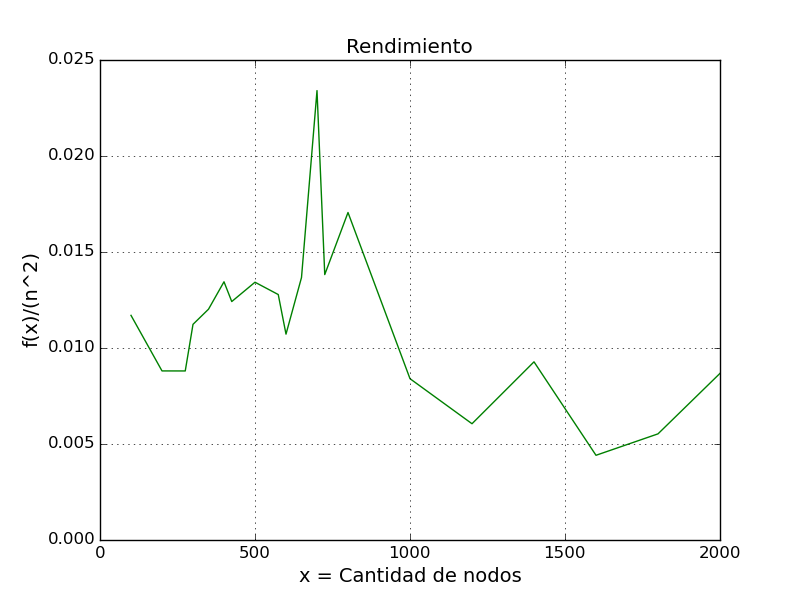
\includegraphics[scale=0.7]{experimentos/bqlocal/rendimiento_aristas_cuadraticas_3/complexity_med_over_n_square.png}
\end{center}

\begin{center}
	\textbf{$y = f(x)/x^3$}\\
	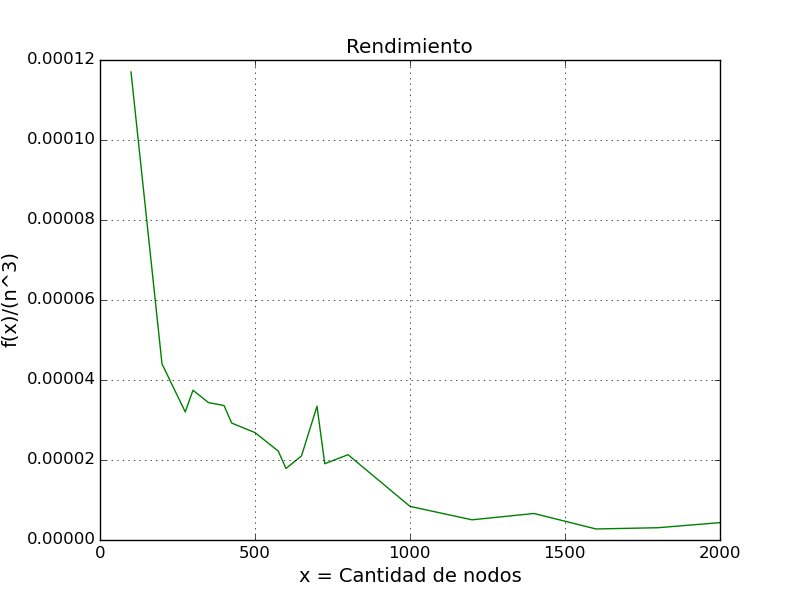
\includegraphics[scale=0.7]{experimentos/bqlocal/rendimiento_aristas_cuadraticas_3/complexity_med_over_n_cube.png}
\end{center}

\begin{center}
	\textbf{$y = f(x)/x^4$}\\
	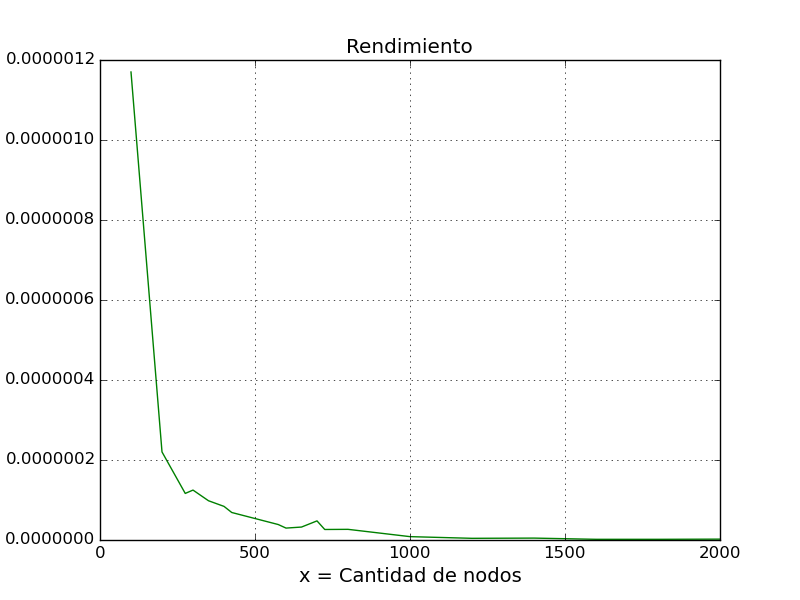
\includegraphics[scale=0.7]{experimentos/bqlocal/rendimiento_aristas_cuadraticas_3/complexity_med_over_n_fourth.png}
\end{center}

Como vemos en las 2 secciones de resultados anteriores, para $n^2$, $n^3$ se mantiene constante dentro de un rango muy reducido en el eje Y, pero para $n^3$ y $n^4$ es una funcion marcadamente decreciente, con lo cual, llegamos a la conclusion de que la curva es o bien,  cuadr\'atica o c\'ubica. Pero analizando con m\'as detalle notamos que la constante para $n^2$ es positiva y un n\'umero razonable (mayor a 1), mientras que la constante de $n^3$ tiende a cero y se aplasta contra el eje X, lo cual es el resultado de dividir una constante por la variable de experimentaci\'on. Con lo cual, al ser $f(x)/x$ creciente,  $f(x)/x^2$ una constante cercana a 10, y $f(x)/x^3$ una curva que tiende a cero, es un buen indicio de que la complejidad te\'orica de $O(n^2)$ es acertada.


\subsection{Experimentacion: Variaci\'on evolutiva de mejora en cada iteracion}
\subsubsection{Rendimiento evolutivo en grafos muy densos}
Resumen del analisis:
\begin{itemize}
	\item Cantidad de tests realizados: 24
	\item Iteraciones promedio: 5
	\item Minima cantidad de iteraciones: 2
	\item Maxima cantidad de iteraciones: 16
\end{itemize}

\begin{center}
	\textbf{Ejemplo de la evoluci\'on en la mejora de la solucion durante las iteraciones de la busqueda local}\\
	\textbf{$y = f(x)$, para cada x=numero de iteracion, f(x) expresa la mejora obtenida en $w_2$ en dicha iteracion}\\
	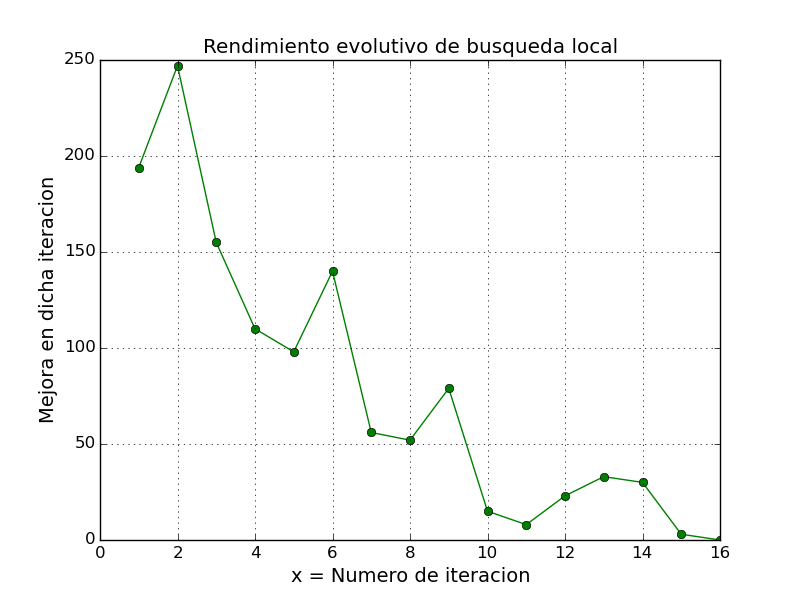
\includegraphics[scale=0.7]{experimentos/bqlocal/rendimiento_evolucion_iteraciones_cliques/test-results/bqlocal/instancia_120_7130_in_iters.png}
\end{center}

En general, todas las funciones son estrictamente decrecientes, salvo excepciones donde en ciertos puntos crece muy poco y vuelve a decrecer mas fuertemente. Esto nos da la pauta de que el grado de mejora en cada iteracion durante la vida del ciclo de la busqueda local decrece a medida que hacemos mas iteraciones, para finalmente estancarse en cero y llegar al criterio de terminaci\'on.

\subsubsection{Rendimiento evolutivo en grafos con densidad lineal de aristas}

Resumen del analisis:
\begin{itemize}
	\item Cantidad de tests realizados: 282
	\item Iteraciones promedio: 2
	\item Minima cantidad de iteraciones: 1
	\item Maxima cantidad de iteraciones: 9
\end{itemize}

Observamos que para grafos menos densos, disminuye la cantidad promedio de iteraciones, esto tambien podr\'ia indicar que hay algun tipo de relacion entre la cantidad de aristas y el cardinal de la vecindad $N$, lo cual tiene sentido, porque a mayor cantidad de aristas en el grafo, mas modificaci\'ones locales pueden hacerse al camino inicial.

\subsection{Experimentacion: Variaci\'on absoluta de w2 en busqueda local}
Otra forma de ponderar el rendimiento de busqueda local es una variaci\'on del analisis realizado en la seccion anterior. Consiste en que, en cada iteracion de busqueda local se almacenen los costos $w_1$ y $w_2$ del camino actual obtenido para luego ser graficado como una funcion donde el eje X consiste en la cantidad de iteraciones y el eje Y denota el valor absoluto del costo. Si realizamos ademas una resta entre el valor inicial y el valor final del eje Y, tendremos cual fue la mejora total del camino. Si realizamos un promedio y una desviacion estandar sobre este ultimo dato, podremos observar para diferentes sets de grafos como es el rendimiento de la busqueda local.















\subsection{Experimentacion: Distintas soluciones iniciales factibles}
Como mencionamos antes, se utiliza Dijkstra sobre $w_1$ para obtener la solucion inicial factible, para comenzar las iteraciones de b\'usqueda local. En esta secci\'on decidimos variar esto y establecer la solucion inicial de busqueda local con la heuristica golosa. Para ciertos grafos preestablecidos que pueden encontrarse en la carpeta \texttt{grafos especiales} las soluciones finales de busqueda local con los 2 modos de solucion inicial son iguales, lo que vari\'o de forma notable fue la cantidad de iteraciones de busqueda local necesarias para llegar a dicha solucion final, debajo se muestra una tabla indicando esto:
\begin{center}
	\begin{tabular}{ | l | c | c |}
	  \hline
	  Grafo especial numero & Cant. iters Dijkstra & Cant. iters Greedy \\
	  \hline
	  Grafo\_1.txt & 3 & 0 \\
	  \hline
	  Grafo\_2.txt & 2 & 0 \\
	  \hline
	  Grafo\_3.txt & 1 & 0 \\
	  \hline
	  Grafo\_4.txt & 0 & 0 \\
	  \hline
	\end{tabular}
\end{center}

Asumimos que esto se debe a la calidad de la soluci\'on provista por el algoritmo goloso.



%Incluye los puntos 3 con GRASP
  \section{Metaheuristica GRASP: Solucion propuesta}

Dado que la metaheur\'istica GRASP es una combinaci\'on entre una heur\'istica golosa aleatorizada y una b\'usqueda local, decidimos utilizar nuestras heur\'isticas previamente mencionadas, con algunas modificaciones.

\subsection{Modificaci\'on a la heur\'istica golosa}

\vspace{2mm}

Durante el ciclo del algoritmo goloso, recordemos que la primera instrucci\'on del ciclo principal, al igual que el algoritmo de Dijkstra, es obtener el m\'inimo nodo de la cola segu\'un $w_2$. En lugar de esto, ahora armamos una lista restringida de canditatos, o RCL. El algoritmo ahora tiene dos par\'ametros, $tipo\_ejecucion$ que indica tres tipos de ejecuci\'on: determin\'istico, por valor y por cantidad, y un par\'ametro $\beta$. El tipo determin\'istico es an\'alogo a la heur\'istica golosa antes descripta, simplemente tomando el m\'inimo y el par\'ametro $\beta$ es ignorado.

\vspace{2mm}

El tipo de ejecuci\'on por valor arma una lista de candidatos filtrados por su valor, seg\'un un porcentaje de alejamiento del valor del m\'inimo, indicado por el par\'ametro $\beta$. Es decir, se toma la cola y se filtran los candidatos factibles cuyo valor sobrepase $(\beta + 1)*valor\_del\_minimo$). Luego se elige al azar uno de los candidatos. 
\vspace{2mm}

El tipo de ejecuci\'on por cantidad se basa en tomar la cola, y tomar los $\beta$ nodos de valor m\'inimo. Luego se elige uno al azar. Como la cola est\'a ordenada, cumple la condici\'on de RCL por cantidad, con lo que basta tomar un n\'umero aleatorio $i$ entre $0$ y  $min\{cola.size(), parametro\_beta\} -1$ y devolver el $i$-\'esimo elemento de la cola.\\
\textbf{Nota: } Los numeros aleatorios generados para elegir de la RCL en un principio se realizaban con los generadores uniformes de c++11, pero dado que en las mediciones se disparaban los tiempos de ejecucion al usar la libreria random, utilizamos el \texttt{rand()} legacy de C con una semilla inicial \texttt{time(NULL)}.
\vspace{2mm}

Por otro lado, el invariante de Dijkstra nos asegura que tomando el mínimo en cada iteraci\'on, podemos sacarlo de la cola y estar seguros de que no volver\'a a ser actualizado (por principio de optimalidad de Bellman aplicado a caminos m\'inimos). El hecho tomar uno aleatorio no nos asegura esto, por lo tanto cada nodo puede ser visitado y encolado m\'as de una vez. En particular cada nodo es encolado tantas veces como pueda ser mejorado por todos sus vecinos, y sin tener alguna tabla de nodos visitados, el algoritmo itera hasta no poder mejorar m\'as ning\'un nodo, momento en el que se vaci\'a la cola y de esa forma llega a la soluci\'on golosa determin\'istica. Notamos esto prematuramente en la experimentaci\'on al obtener resultados id\'enticos entre la heur\'stica golosa normal y aleatorizada en absolutamente todos los casos y decidimos solucionarlo marcando cada vez que un nodo ingresa en la cola de prioridad y restringirlo a una sola vez, mediante un $vector<bool>$. De esta forma nos aseguramos de esto, y una vez implementada esta mejora, comenzamos a obtener soluciones distintas entre ambos algoritmos, y pudimos ver distintos resultados al variar el par\'ametro $\beta$ (mientras m\'as pequeno, m\'as se acerca al resultado determin\'istico).

\vspace{2mm}

\begin{algorithmic}

\While{ $ !cola=\emptyset$ }
	\If{$tipo\_ejecucion == deterministico$}
    	 \State $nodo \: minimo = minimo(cola)$    
    \ElsIf{$tipo\_ejecucion == por\_cantidad$}
		\State $int \: random = random(0, min\{cola.size(), parametro\_beta\} -1)$
		\State $ \: minimo = cola[random]$
		\Comment $O(random)$, no es iterador de acceso aleatorio
	\ElsIf{$tipo_ejecucion == por\_valor$}
		\State $lista \: nodo \: candidatos = \emptyset$
		\State $int \: i = 0$
		\While{$i<tamano(cola)$}
			\If{$ cola[i] \leq valor\_limite $}
				\State $ agregar(cola[i], candidatos) $
			\EndIf
		\EndWhile
		\State $int \: random = random(0, min\{cola.size(), parametro\_beta\} -1)$
		\State $ \: minimo = candidatos[random]$
		\State $visitados[minimo] = true$
		\EndIf
		
\EndWhile
\end{algorithmic}

\vspace{2mm}

No fue necesario realizar modificaciones a la heur\'istica de b\'usqueda local.

\subsection{Critero de terminaci\'on}

Fijada ya la heur\'istica golosa aleatorizada, y la heur\'istica de b\'usqueda local, queda definir por el criterio de terminaci\'on.

\vspace{2mm}

Hay dos criterios implementados:

\begin{enumerate}
\item Cantidad de iteraciones l\'imite (fijo o variable)
\item Cantidad de iteraciones sin mejora consecutivas
\end{enumerate}

Cantidad de iteraciones l\'imite, como su nombre lo indica itera hasta un l\'imite dado, ya sea una constante, o una variable del problema, por ejemplo la cantidad de nodos del grafo. Cantidad iteraciones sin mejora corta la iteraci\'on cuando se haya alcanzado una cantidad de iteraciones m\'inimas sin que haya habido alguna mejora en el camino.

\vspace{2mm}

\subsection{Consideraciones}

Dada la naturaleza aleatoria de la heur\'istica greedy aleatorizada, en una cantidad de casos despreciable en cuanto al total de experimentos (pero aun as\'i, ocurrieron), la heur\'istica, a\'un habiendo un camino factible en el grafo, no pudo proporcionar una soluci\'on. Por esto, decidimos validar la soluci\'on obtenida del algoritmo goloso, y en caso de que no sea v\'alida, ejecutarlo nuevamente hasta llegar a un tope de iteraciones fijo. Superado este tope de iteraciones, ajustamos el par\'ametro $\beta$ de GRASP, en el caso de que la b\'usqueda golosa sea por cantidad, lo decrementamos en $1$, en el caso por valor, simplemente lo fijamos en $0$ lo cual equivale a la b\'uqueda golosa determin\'istica.

\subsection{Pseudoc\'odigo}

Nota: la entrada $criterios$ se refiere a las variables:

\begin{enumerate}
\item $tipo\_golosa$ : el tipo de ejecuci\'on para la parte golosa.
\item $tipo\_bq$ : el tipo de ejecuci\'on para la b\'usqueda local
\item $\beta$ : el par\'ametro para armar la RCL de la parte golosa.
\item $citerio\_terminacion$ : el criterio de terminaci\'on de GRASP.
\item $max\_its$ : la cantidad de iteraciones l\'mite del primer criterio de terminaci\'on.
\item $max\_its\_sin\ _mejora$ : la cantidad de iteraciones en la cual el segundo criterio debe cortar el algoritmo sin obtener mejora.
\item $bad\_rgreedy\_its$ : la cantidad de iteraciones consecutivas para las cuales corremos la heur\'istica golosa aleatorizada hasta que de una soluci\'on factible.
\end{enumerate}

\begin{algorithmic}[1]

\Procedure{$Sol\_GRASP$}{$Grafo\: g, \:vertice\: v_1,\: vertice \: v_2, \: int \: k, criterios$}{$\rightarrow lista<eje>\: camino$}

	\Statex
	\State $bool \: condicion\_terminacion\: =\: false$
    \State $lista<eje> \:mejor\_solucion\: = \emptyset$
    \State $int \:costo\_mejor\_solucion\: =\: \inf$
    \State $lista<eje> \:camino\: = \emptyset$
    \State $int\: cant\_iters \:= \:0$
    \State $int\: cant\_iters\_sin\_mejora \:= 0$
    \State $int\: cant\_iters\_sin\_sol\_rgreedy\_factible = 0$
    \State $ bool\: sol\_valida\_rgreedy\: =\: false $
    \State $vector<pair<int, costo> > \: mejora\_iters\_grasp$
    \Statex 

    \While{$!condicion\_terminacion$}

    	\State $camino\: =\: solucion\_golosa(g, v_1,v_2, tipo\_golosa, \beta)$
    	\State $ sol\_valida\_rgreedy= validar\_solucion(camino)$
    	\Comment{Obtenemos solucion greedy}

    	\Statex
    	\If{$hay solucion$}
    		\If{$sol\_valida\_rgreedy$}
    		\Comment{Validamos si es factible}
	
	    			\State $cant\_iters\_sin\_sol\_rgreedy\_factible = 0$
	
	    			\State $int\: mejora\_iteracion\_actual\: = 0$
	        	    \State $int\: cant\_iters\_bqlocal\: = 0$
	
	        	    \Statex
	
	    			\While{$mejora\_iteracion\_actual > 0$}
	    					\Comment{Aplicamos Busqueda Local}
	    					\State $mejora\_iteracion\_actual=busqueda\_local(g, tipo\_bq, camino)$
	    					\State $cant\_iters\_bqlocal++$
	
	    			\EndWhile
	
	    			\State $ int \:  costo\_sol\_actual \: = \: costo\_w_2(camino)$
	
	    			\Statex
	
					\If{$costo\_sol\_actual < costo\_mejor\_solucion$}
					\Comment{Reemplazamos si es mejor solucion}
	
						\If{$cant\_iters>0$}
							\State $ agregar(mejora\_iters\_grasp, par<cant\_iters, costo\_mejor\_solucion - costo\_solucion\_actual>) $
						\EndIf
	        	    	\State $costo\_mejor\_solucion = costo\_sol\_actual$
	        	    	\State $mejor\_solucion = camino$
	        	    
	        	   	    \State $cant\_iters\_sin\_mejora = 0$
	        		\Else
	        			\If{$cant\_iters>0$}
	        				\State $ agregar(mejora\_iters\_grasp, par<cant\_iters, 0)>) $
	        	        \EndIf
	        	        \State $cant\_iters\_sin\_mejora++$
	        	    
	        	    	
	        	\EndIf
	
	        	\State $cant\_iters++$
	    	
	    	    	\Else
	    	    	\Comment{$sol\_valida\_rgreedy = false$}
	    	    	\State $cant\_iters\_sin\_sol\_greedy\_rand\_factible++$
	    	    	\If{$cant\_iters\_sin\_sol\_greedy\_rand\_factible\geq bad\_rgreedy\_its$}
	    	    		\If{$tipo\_golosa == por\_cantidad$}
	    	    		\Comment Maximo de its de greedy sin Solucion
	    	    	            \If{$parametro\_beta\geq2$}
	    	    	            	\Comment Ajustamos parametros de GRASP
	    	    	                \State $parametro\_beta--$
	    	    	            \EndIf
	    	    	    \ElsIf{$tipo\_golosa == por\_valor$}
	
	        	    	\State $parametro_beta = 0$
	        		\EndIf
	        		\State $cant\_iters\_sin\_sol\_greedy\_rand\_factible = 0$
	        	\EndIf
        	\EndIf
        \Else
        \Comment No hay Solucion
        	\State $break$
        \EndIf	
    \If{$criterio\_terminacion == 1$}
    \Comment{Si se cumple el criterio de terminacion}
           \State $condicion\_terminacion = (cant\_iters < max\_its)$            
        \ElsIf{$criterio\_terminacion == 2$}
            \State $condicion_terminacion = (cant\_iters\_sin\_mejora < max\_its\_sin\ _mejora)$
        \EndIf

       \EndWhile

       \State $return\:  mejor\_solucion$

\EndProcedure
\end{algorithmic}


\subsection{An\'alisis de complejidad}

A continuaci\'on realizaremos el an\'alisis de complejidad te\'orica de una iteraci\'on de la metaheur\'istica GRASP.
\vspace{2mm}


 Dentro del ciclo principal, la primera instrucci\'on es generar una soluci\'on golosa aleatorizada inicial. La complejidad de la heur\'istica golosa determin\'istica es de $O(n^2 + m log n)$. La heur\'istica golosa aleatorizada difiere de la determin\'istica en la elecci\'on del nodo a desencolar, en caso de ser RCL por cantidad, extraer un elemento random de la cola cuesta $(avanzar\: el\: iterador\: de\: la \:cola \:min\{\beta, n\}\:veces)+O(1) eliminar$, en caso de ser por valor, se filtra toda la cola, por lo que cuesta $O(n)$. El hecho de marcar los nodos y encolarlos una sola vez nos indica que el ciclo $while$ externo itera $n$ veces.

\vspace{2mm}
   
   El ciclo $for$ interno no recibi\'o modificaciones excepto por un condicional que se ejecuta en tiempo constante. El peor de los casos se da cuando la cota $K$ es de mayor peso a cualquier camino simple del grafo y este condicional es siempre verdadero, por lo que el ciclo se vuelve an\'alogo al de Dijkstra y ejecuta en $O(mlogn)$ (sabemos que cada arista se analiza una vez porque marcamos los nodos).

\vspace{2mm}

Por lo tanto en caso de ser RCL por valor la complejidad es de: $O(n^2 + m * logn + \beta * n )$ y en caso de ser por valor es de $O(n^2 + m log n)$. El par\'ametro $\beta$ puede ser acotado por $n$, dado que nunca va a poder armarse una RCL con m\'as de $n$ candidatos, ya que cada nodo est\'a en la cola a lo sumo una vez, con lo cual la complejidad de la heur\'istica aleatorizada no difere de la determin\'istica.


\vspace{2mm}

Acto seguido se valida si esta soluci\'on es factible, en tiempo constante, se declaran enteros y se procede a ejecutar la b\'usqueda local, cuya complejidad es de $O(k*n^2)$, siendo $k$ la cantidad de iteraciones hasta cumplida la condici\'on de terminaci\'on. Lo que resta son simplemente condicionales y asignaciones de tiempo constante, lo que nos da un resultado de $O(n^2 + m log n + k*(n^2)$.

\subsection{Experimentacion: Mediciones de Performance}

A continuacion presentamos los resultados de los experimentos, an\'alogos a los de los algoritmos anteriores, con la salvedad de que para las mismas instancias de grafos, analizaramos primero con RCL por cantidad, con $\beta=n$(peor caso), y luego con RCL por valor, con $\beta=$

\subsubsection{Rendimiento para grafos con densidad cuadratica de aristas}
\begin{itemize}
	\item cant nodos min = $200$
	\item cant nodos max = $350$
	\item peso maximo w1 = $250$
	\item peso maximo w2 = $400$
	\item step nodos = $25$
	\item step aristas = $2500$
	\item aristas minimas = $\frac{n*(n-1)}{8}$
	\item aristas maximas = $\frac{n*(n-1)}{3}$
\end{itemize}								

\begin{center}
	\textbf{Tiempo de ejecuci\'on en microsegundos para esta familia}\\
	\textbf{$y = f(x)$}\\
	\includegraphics[scale=0.7]{experimentos/resultados_tiempo_grasp_cliques/{grasp.tmpplot_complexity_variation}.png}
\end{center}

\begin{center}
	\textbf{$y = f(x)/x$}\\
	\includegraphics[scale=0.7]{experimentos/resultados_tiempo_grasp_cliques/{grasp.tmpplot_complexity_med_over_n}.png}
\end{center}

\begin{center}
	\textbf{$y = f(x)/x^2$}\\
	\includegraphics[scale=0.7]{experimentos/resultados_tiempo_grasp_cliques/{grasp.tmpplot_complexity_med_over_n_square}.png}
\end{center}

\begin{center}
	\textbf{$y = f(x)/x^3$}\\
	\includegraphics[scale=0.7]{experimentos/resultados_tiempo_grasp_cliques/{grasp.tmpplot_complexity_med_over_n_cube}.png}
\end{center}

\begin{center}
	\textbf{$y = f(x)/x^4$}\\
	\includegraphics[scale=0.7]{experimentos/resultados_tiempo_grasp_cliques/{grasp.tmpplot_complexity_med_over_n_fourth}.png}
\end{center}


\subsubsection{Rendimiento para grafos con densidad lineal de aristas}
\begin{itemize}
	\item cant nodos min = $200$
	\item cant nodos max = $2000$
	\item peso maximo w1 = $200$
	\item peso maximo w2 = $200$
	\item step nodos = $200$
	\item step aristas = $2500$
	\item aristas minimas = $n-1$
	\item aristas maximas = $10*n$
\end{itemize}								
\begin{center}
	\textbf{Tiempo de ejecuci\'on en microsegundos para esta familia}\\
	\textbf{$y = f(x)$}\\
	\includegraphics[scale=0.7]{experimentos/resultados_tiempo_grasp_cliques/{grasp.tmpplot_complexity_variation}.png}
\end{center}

\begin{center}
	\textbf{$y = f(x)/x$}\\
	\includegraphics[scale=0.7]{experimentos/resultados_tiempo_grasp_cliques/{grasp.tmpplot_complexity_med_over_n}.png}
\end{center}

\begin{center}
	\textbf{$y = f(x)/x^2$}\\
	\includegraphics[scale=0.7]{experimentos/resultados_tiempo_grasp_cliques/{grasp.tmpplot_complexity_med_over_n_square}.png}
\end{center}

\begin{center}
	\textbf{$y = f(x)/x^3$}\\
	\includegraphics[scale=0.7]{experimentos/resultados_tiempo_grasp_cliques/{grasp.tmpplot_complexity_med_over_n_cube}.png}
\end{center}

\begin{center}
	\textbf{$y = f(x)/x^4$}\\
	\includegraphics[scale=0.7]{experimentos/resultados_tiempo_grasp_cliques/{grasp.tmpplot_complexity_med_over_n_fourth}.png}
\end{center}

\subsection{Experimentaci\'on de optimalidad}

A continuaci\'on los experimentos de an\'alisis de soluci\'on de la metaheur\'istica, comparada con el algoritmo exacto y las dem\'as. Para estos experimentos adem\'as, fijando un costo $w_1$ m\'aximo a las aristas, variamos la cota $K$ de los grafos para verificar optimalidad-
\subsubsection{Optimalidad para grafos lineales con $w1 = 120$}
\begin{itemize}
	\item cant nodos min = $200$
	\item cant nodos max = $2000$
	\item peso maximo w1 = $250$
	\item peso maximo w2 = $400$
	\item limit w1 = $120$
	\item step nodos = $100$
	\item step aristas = $2500$
	\item aristas minimas = $2*n$
	\item aristas maximas = $20*n$
\end{itemize}			

\begin{center}
	\includegraphics[scale=0.7]{experimentos/optimalidad_lineal_grasp_120/{comparacion_optimalidad}.png}
\end{center}

\subsubsection{Optimalidad para grafos lineales con $w1 = 200$}
\begin{itemize}
	\item cant nodos min = $200$
	\item cant nodos max = $2000$
	\item peso maximo w1 = $250$
	\item peso maximo w2 = $400$
	\item limit w1 = $200$
	\item step nodos = $100$
	\item step aristas = $2500$
	\item aristas minimas = $2*n$
	\item aristas maximas = $20*n$
\end{itemize}			

\begin{center}
	\includegraphics[scale=0.7]{experimentos/optimalidad_lineal_grasp_200/{comparacion_optimalidad}.png}
\end{center}

\begin{lstlisting}[frame=single]
Cantidad de tests realizados: 56
Tiempo promedio microsegundos heuristica: 63565.671
Tiempo promedio microsegundos exacto: 31439.678
Porcentaje de aciertos(cantidad de veces que GRASP da la sol exacta/cantidad de tests hechos): 14.285
Porcentaje de alejamiento de la heuristica a la solucion exacta promedio entre grasp y exacta: 109.460
Desviacion estandar del alejamiento de la heuristica a la solucion exacta promedio entre grasp y exacta: 121.493
Minimo alejamiento porcentual entre grasp y exacta: 0
Maximo alejamiento porcentual entre grasp y exacta: 522.400

\end{lstlisting}

\subsubsection{Optimalidad para grafos cuadr\'aticos con $w1 = 150$}
\begin{itemize}
	\item cant nodos min = $10$
	\item cant nodos max = $260$
	\item peso maximo w1 = $250$
	\item peso maximo w2 = $400$
	\item limit w1 = $150$
	\item step nodos = $25$
	\item step aristas = $5000$
	\item aristas minimas = $(n * (n-1))=/12$
	\item aristas maximas = $n * (n-1))=/2$
\end{itemize}			

\begin{center}
	\includegraphics[scale=0.7]{experimentos/optimalidad_cliques_grasp_150/{comparacion_optimalidad}.png}
\end{center}

\begin{lstlisting}[frame=single]
Cantidad de tests realizados: 26
Tiempo promedio microsegundos heuristica: 2877.366
Tiempo promedio microsegundos exacto: 5129.884
Porcentaje de aciertos(cantidad de veces que GRASP da la sol exacta/cantidad de tests hechos): 42.307
Porcentaje de alejamiento de la heuristica a la solucion exacta promedio entre grasp y exacta: 50.108
Desviacion estandar del alejamiento de la heuristica a la solucion exacta promedio entre grasp y exacta: 69.2576
Minimo alejamiento porcentual entre grasp y exacta: 0
Maximo alejamiento porcentual entre grasp y exacta: 259.600
\end{lstlisting}


\subsubsection{Optimalidad para grafos cuadr\'aticos con $w1 = 120$}
\begin{itemize}
	\item cant nodos min = $10$
	\item cant nodos max = $260$
	\item peso maximo w1 = $250$
	\item peso maximo w2 = $400$
	\item limit w1 = $120$
	\item step nodos = $25$
	\item step aristas = $5000$
	\item aristas minimas = $(n * (n-1))=/12$
	\item aristas maximas = $n * (n-1))=/2$
\end{itemize}			

\begin{center}
	\includegraphics[scale=0.7]{experimentos/optimalidad_cliques_grasp_120/{comparacion_optimalidad}.png}
\end{center}
\begin{lstlisting}[frame=single]
Cantidad de tests realizados: 26
Tiempo promedio microsegundos heuristica: 2751.938
Tiempo promedio microsegundos exacto: 4685.692
Porcentaje de aciertos(cantidad de veces que GRASP da la sol exacta/cantidad de tests hechos): 53.846
Porcentaje de alejamiento de la heuristica a la solucion exacta promedio entre grasp y exacta: 81.088
Desviacion estandar del alejamiento de la heuristica a la solucion exacta promedio entre grasp y exacta: 189.693
Minimo alejamiento porcentual entre grasp y exacta: 0
Maximo alejamiento porcentual entre grasp y exacta: 789.400
\end{lstlisting}

Estas pruebas fueron resueltas con el objetivo de analizar como vari\'an las soluciones de la heur\'istica segu\'n los caminos factibles que delimita la cota $K$. A continuaci\'on, fijaremos la cota $K$ en $120$ (que fue la que mostr\'o soluciones m\'as interesates en la pr\'actica) y variaremos el par\'ametro $\beta$, por cantidad y luego por valor. Condensaremos las familias de an\'alisis en un mismo gr\'afico, y las corremos sobre un mismo conjunto de instancias.

\subsubsection{Optimalidad para grafos con RCL por cantidad}

\begin{itemize}
	\item cant nodos min = $10$
	\item cant nodos max = $260$
	\item peso maximo w1 = $250$
	\item peso maximo w2 = $400$
	\item limit w1 = $150$
	\item step nodos = $25$
	\item step aristas = $20000$
	\item aristas minimas = $n$
	\item aristas maximas = $n * (n-1))=/2$
\end{itemize}


$\beta= n/4$
\begin{lstlisting}[frame=single]
Cantidad de tests realizados: 13
Tiempo promedio microsegundos heuristica: 4781.004
Tiempo promedio microsegundos exacto: 15248.461
Porcentaje de aciertos(cantidad de veces que GRASP da la sol exacta/cantidad de tests hechos): 38.461
Porcentaje de alejamiento de la heuristica a la solucion exacta promedio entre grasp y exacta: 68.915
Desviacion estandar del alejamiento de la heuristica a la solucion exacta promedio entre grasp y exacta: 116.131
Minimo alejamiento porcentual entre grasp y exacta: 0
Maximo alejamiento porcentual entre grasp y exacta: 396.900
\end{lstlisting}
$\beta=n/32$
\begin{lstlisting}[frame=single]
Cantidad de tests realizados: 13
Tiempo promedio microsegundos heuristica: 4558.685
Tiempo promedio microsegundos exacto: 14349.692
Porcentaje de aciertos(cantidad de veces que GRASP da la sol exacta/cantidad de tests hechos): 38.461
Porcentaje de alejamiento de la heuristica a la solucion exacta promedio entre grasp y exacta: 21.646
Desviacion estandar del alejamiento de la heuristica a la solucion exacta promedio entre grasp y exacta: 28.0819
Minimo alejamiento porcentual entre grasp y exacta: 0
Maximo alejamiento porcentual entre grasp y exacta: 78.100
\end{lstlisting}
$\beta=n/64$
\begin{lstlisting}[frame=single]
Cantidad de tests realizados: 13
Tiempo promedio microsegundos heuristica: 4516.103
Tiempo promedio microsegundos exacto: 14427.461
Porcentaje de aciertos(cantidad de veces que GRASP da la sol exacta/cantidad de tests hechos): 46.153
Porcentaje de alejamiento de la heuristica a la solucion exacta promedio entre grasp y exacta: 16.130
Desviacion estandar del alejamiento de la heuristica a la solucion exacta promedio entre grasp y exacta: 23.74
Minimo alejamiento porcentual entre grasp y exacta: 0
Maximo alejamiento porcentual entre grasp y exacta: 72.000
\end{lstlisting}

Vemos que variar el par\'ametro $\beta$ y dividi\'endolo sucesivamente por potencias de dos va a justando el alejamiento de los no aciertos y aumenta la cantidad de aciertos.

\vspace{2mm}


Para un experimento en particular $\beta = n/128$, vemos que iguala en cantidad de aciertos a la heur\'istica golosa y reduce el alejamiento de los no aciertos.
\begin{itemize}
	\item cant nodos min = $10$
	\item cant nodos max = $280$
	\item peso maximo w1 = $250$
	\item peso maximo w2 = $400$
	\item limit w1 = $150$
	\item step nodos = $25$
	\item step aristas = $20000$
	\item aristas minimas = $n$
	\item aristas maximas = $n * (n-1))=/2$
\end{itemize}



\begin{lstlisting}[frame=single]
Golosa:
Porcentaje de aciertos(cantidad de veces que GOLOSA da la sol exacta/cantidad de tests hechos): 83.018
Porcentaje de alejamiento de la heuristica a la solucion exacta promedio entre golosa y exacta: 4.990
Desviacion estandar del alejamiento de la heuristica a la solucion exacta promedio entre golosa y exacta: 18.1754
GRASP:
Porcentaje de aciertos(cantidad de veces que GRASP da la sol exacta/cantidad de tests hechos): 83.018
Porcentaje de alejamiento de la heuristica a la solucion exacta promedio entre grasp y exacta: 3.611
Desviacion estandar del alejamiento de la heuristica a la solucion exacta promedio entre grasp y exacta: 12.1007
\end{lstlisting}[frame=single]

Ahora variamos $\beta$ en RCL por valor

$\beta = 0.9$
\begin{lstlisting}[frame=singl
Cantidad de tests realizados: 14
Tiempo promedio microsegundos heuristica: 4620.666
Tiempo promedio microsegundos exacto: 13796.214
Porcentaje de aciertos(cantidad de veces que GRASP da la sol exacta/cantidad de tests hechos): 64.285
Porcentaje de alejamiento de la heuristica a la solucion exacta promedio entre grasp y exacta: 18.246
Desviacion estandar del alejamiento de la heuristica a la solucion exacta promedio entre grasp y exacta: 44.6027
Minimo alejamiento porcentual entre grasp y exacta: 0
Maximo alejamiento porcentual entre grasp y exacta: 175.000
\end{lstlisting}[frame=single]

$beta = 0.8$
\begin{lstlisting}[frame=singl
Cantidad de tests realizados: 14
Tiempo promedio microsegundos heuristica: 4600.035
Tiempo promedio microsegundos exacto: 14057.071
Porcentaje de aciertos(cantidad de veces que GRASP da la sol exacta/cantidad de tests hechos): 71.428
Porcentaje de alejamiento de la heuristica a la solucion exacta promedio entre grasp y exacta: 3.376
Desviacion estandar del alejamiento de la heuristica a la solucion exacta promedio entre grasp y exacta: 5.34277
Minimo alejamiento porcentual entre grasp y exacta: 0
Maximo alejamiento porcentual entre grasp y exacta: 17.000
\end{lstlisting}[frame=single]

$\beta = 0.6$

\begin{lstlisting}[frame=singl
\begin{}
Cantidad de tests realizados: 14
Tiempo promedio microsegundos heuristica: 4568.095
Tiempo promedio microsegundos exacto: 13775.857
Porcentaje de aciertos(cantidad de veces que GRASP da la sol exacta/cantidad de tests hechos): 78.571
Porcentaje de alejamiento de la heuristica a la solucion exacta promedio entre grasp y exacta: 2.615
Desviacion estandar del alejamiento de la heuristica a la solucion exacta promedio entre grasp y exacta: 5.04769
Minimo alejamiento porcentual entre grasp y exacta: 0
Maximo alejamiento porcentual entre grasp y exacta: 17.000
\end{lstlisting}[frame=single]

Vemos como tambi\'en reducir el valor l\'mite causa que no s\'olo produzca m\'as aciertos sino que tambi\'en sus no aciertos se ajustan m\'as.
%---------------	-----------------------------------------------------------------------------------------------------------------
%te dejo un poco de data aca
%esto es en cliques:
%(carpeta: informe/experimentos/performance-optimalidad-cliques_beta_n_over_128/)
%el resto piolon, igual hace otros experimentos(tienen que ser distintos experimentos el 3d y el pto 4), pero conclui que el posta es n/128 
%
%Golosa:
%	Porcentaje de aciertos(cantidad de veces que GOLOSA da la sol exacta/cantidad de tests hechos): 83.018
%	Porcentaje de alejamiento de la heuristica a la solucion exacta promedio entre golosa y exacta: 4.990
%	Desviacion estandar del alejamiento de la heuristica a la solucion exacta promedio entre golosa y exacta: 18.1754
%GRASP:
%	Porcentaje de aciertos(cantidad de veces que GRASP da la sol exacta/cantidad de tests hechos): 83.018
%	Porcentaje de alejamiento de la heuristica a la solucion exacta promedio entre grasp y exacta: 3.611
%	Desviacion estandar del alejamiento de la heuristica a la solucion exacta promedio entre grasp y exacta: 12.1007
%
%Da lo mismo que golosa en efectividad pero fijate que aca GRASP da mas cercano y con menor dispersion al optimo. :D :D :D
%
%--------------------------------------------------------------------------------------------------------------------------------


%explica y detalla como se realizaron los experimentos, casos de prueba y mediciones, y que graficos se realizaron
%punto 4 del tp
\section{Experimentacion General}
En esta secci\'on analizaremos la calidad de las heuristicas mediante la comparaci\'on y analisis estadistico de las soluciones, asi tambien el tiempo insumido en obtener dichas soluciones, para diferentes grupos de instancias de grafos generados al azar.

\subsection{Generacion de conjuntos de grafos aleatorios}

\subsubsection{Generador de grafos aleatorios}
El generador aleatorio de grafos es un binario aparte de los algoritmos, que recibe como parametros
\begin{itemize}
\item cantidad de nodos
\item cantidad de aristas
\item peso minimo $w_1$
\item peso maximo $w_1$
\item peso minimo $w_2$
\item peso maximo $w_2$
\item limite $w_1$
\end{itemize}
y devuelve por salida estandar una instancia del problema tal como esta especificado el formato de entrada en el enunciado de este TP.\\
\textbf{Nota: }Los generadores de numeros aleatorios de este generador de grafos tienen distribucion uniforme(Usan random de C++11).

\vspace{1cm}

La generaci\'on del grafo se realiza de la siguiente manera: 
Sean n=\{cantidad de nodos del grafo\} y m=\{cantidad de aristas\}, se inicializa un vector $aristas =  <(0, 1), ..., (0, n-1), (1, 2), ..., (1, n-1), ..., (n - 2, n-1)>$ conteniendo todas las aristas posibles en el grafo(notar que como no es digrafo, no se repiten aristas simetricas, ni tampoco de asignan self-loops).

\vspace{1cm}

Luego se mezcla aleatoriamente este vector usando el \texttt{Algoritmo de Shuffle de Knuth o Fisher Yates Shuffle} y se imprime la cabecera del grafo a la salida estandar conteniendo los nodos origen, destino y el parametro k generados como numeros aleatorios uniformes. Ahora basta tomar la cantidad m de aristas requeridas por par\'ametro y serializar la salida linea por linea, nuevamente generando numeros aleatorios con distribucion uniforme sobre los rangos de pesos $w_1$ y $w_2$ pasados por par\'ametro. Finalmente se imprime un 0 indicando el final de la entrada.

\subsubsection{Script generador de conjuntos de grafos}
Se realizo un script el cual genera conjuntos de grafos usando el generador de la seccion anterior, basicamente, se setean dos rangos, de cantidad de nodos y cantidad de aristas, y los parametros fijos como limite $w_1$, limites de los pesos, etc. El script genera iterativamente el conjunto de grafos llamando repetidamente al generador, notemos que podemos(y es lo que hicimos en los experimentos), poner la cantidad de aristas en funcion de la cantidad de nodos y de esta forma poder determinar la densidad de los conjuntos de grafos generados.

\subsection{Scripts de optimalidad - Calculo de puntajes y estadisticas}
Se realizaron diversos scripts para automatizar el analisis de optimalidad y performance, vamos a analizar el script de optimalidad que se ejecuto para obtener los resultados de esta secci\'on.\\
Se trata de un script en bash que para cada instancia del conjunto de grafos generados aleatoriamente, ejecuta los 4 algoritmos (exacta, golosa, busqueda local, grasp) y va realizando calculos estadisticos de los resultados obtenidos, tanto de la solucion como del tiempo consumido para obtenerla.
Los analisis estadisticos que se realizan son:\\
\begin{itemize}
	\item Tiempo promedio microsegundos consumido por el algoritmo
	\item Porcentaje de veces que la heuristica da la solucion optima
	\item Desviacion estandar de veces que la heuristica da la sol. optima
	\item Lejan\'ia promedio de la solucion obtenida a la solucion optima
	\item Desviacion estandar de la lejan\'ia de las soluciones entre la obtenida y la optima
	\item Minima y maxima lejan\'ia obtenida en este conjunto de instancias
\end{itemize}

\textbf{Nota: }La lejan\'ia entre 2 soluciones se mide haciendo el siguiente calculo: 
$ 100 *(\frac{solucionHeuristica}{solucionOptima} - 1)  $ que indica en porcentaje cual es el ratio de distancia entre los dos valores del cociente.\\
\textbf{Nota: } Los calculos estadisticos (promedio y desviacion estandar) se realizan sobre la lista de resultados obtenida de la ejecucion secuencial y el calculo de la lejania mencionado aqui arriba para cada uno de los algoritmos(exacto y heuristica) sobre cada instancia del conjunto de pruebas.

Podemos considerar una especie de puntuacion asignada a cada heuristica viendo el porcentaje de optimalidad y tambien podemos analizar, que cuando no da la solucion optima, la lejania a la optima, con cierta dispersion sea adecuada, segun el problema y el las necesidades del contexto donde se aplica.

\subsection{Scripts de optimalidad - Graficos de optimalidad comparativos}
El script de optimalidad tambien realiza un grafico, en el cual puede verse en el eje X la cantidad de nodos de la instancia y en el eje Y, \texttt{un promedio de los pesos $w_2$ de soluciones para la variacion de aristas para esa cantidad de nodos} de cada algoritmo corrido, distintas referencias y colores indican para cada cantidad de nodos, el valor $w_2$ de las soluciones obtenidas, en este grafico podemos apreciar la distribucion de las soluciones sobre el eje Y a medida que var\'ia la cantidad de nodos.\\
\textbf{Referencias del gr\'afico: } Los triangulos azules representan las soluciones de busqueda local, los signos + amarillos, representan las soluciones del algoritmo exacto, los cuadrados verdes simbolizan las soluciones del algoritmo goloso, y los asteriscos rojos representan las soluciones de GRASP.

\subsection{Calidad de las heuristicas respecto a la soluci\'on exacta}
Se corrieron los scripts de optimalidad con diferentes conjuntos de instancias de grafos aleatorios, y se realizaron los gr\'aficos y el analisis estad\'istico correspondiente, a continuacion se presentan los resultados.
\subsubsection{Comparacion Exacta-Golosa-Busqueda Local}
Se eligieron, 3 diferentes densidades de grafos, y se corrieron los algoritmos con los scripts mencionados anteriormente, a continuacion presentamos los resultados estadisticos, asi tambien como los gr\'aficos.

\subsubsection{Grafos aleatorios de baja densidad de aristas}
\textbf{Parametros del experimento:}
\begin{itemize}
	\item Parametro Beta GRASP: $\frac{cantNodos}{128}$
	\item Cantidad de grafos analizados: 71
	\item Cantidad minima de nodos: 100
	\item Cantidad maxima de nodos: 1800
	\item Rango peso $w_1$: [0..250]
	\item Rango peso $w_2$: [0..400]
	\item Cota de $w_1$: 200
	\item Cantidad minima de aristas: $n-1$
	\item Cantidad maxima de aristas: $10*n$
\end{itemize}

\vspace{1cm}

\textbf{Resultados del analisis (Golosa):}
\begin{lstlisting}[frame=single]	
	Tiempo promedio microsegundos heuristica: 19636.985
	Tiempo promedio microsegundos exacto: 16899.281
	Heuristica da la solucion optima: 98.591% de los casos
	Lejania promedio de la heuristica a la solucion optima: 0.261%
	Desv. estandar de la lejania entre las soluciones: 2.19181
	Minima lejania entre bqlocal y exacta: 0
	Maxima lejania entre bqlocal y exacta: 18.600%
\end{lstlisting}

\textbf{Resultados del analisis (Busqueda local):}
\begin{lstlisting}[frame=single]	
	Tiempo promedio microsegundos heuristica: 8091.119
	Tiempo promedio microsegundos exacto: 16899.281
	Heuristica da la solucion optima: 32.394% de los casos
	Lejania promedio de la heuristica a la solucion optima: 87.626%
	Desv. estandar de la lejania entre las soluciones: 118.585
	Minima lejania entre bqlocal y exacta: 0
	Maxima lejania entre bqlocal y exacta: 662.700%
\end{lstlisting}

\textbf{Resultados del analisis (Metaheuristica GRASP):}
\begin{lstlisting}[frame=single]	
	Tiempo promedio microsegundos heuristica: 26709.723
	Tiempo promedio microsegundos exacto: 16899.281
	Heuristica da la solucion optima: 57.746% de los casos
	Lejania promedio de la heuristica a la solucion optima: 33.373%
	Desv. estandar de la lejania entre las soluciones: 70.8898
	Minima lejania entre bqlocal y exacta: 0
	Maxima lejania entre bqlocal y exacta: 453.300%
\end{lstlisting}

\vspace{2cm}

\begin{center}	
	\textbf{Distribucion de los resultados}\\
	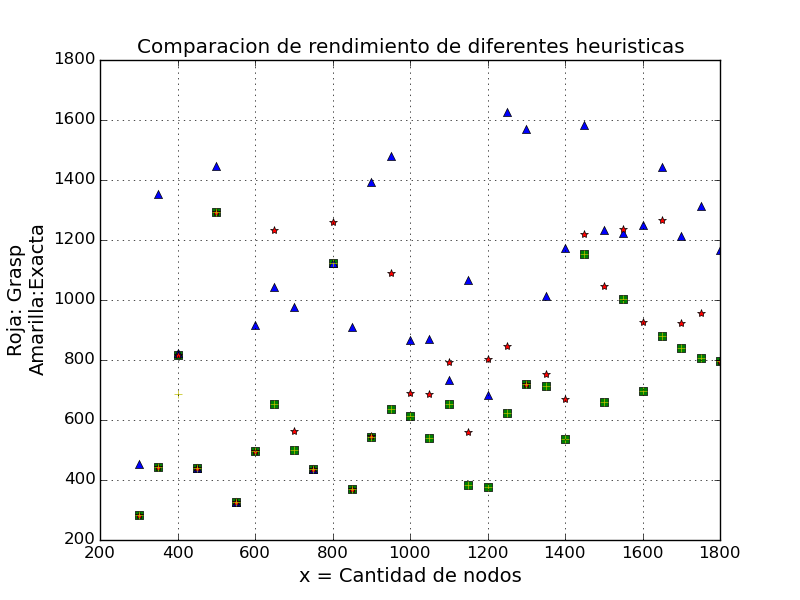
\includegraphics[scale=0.7]{experimentos/performance-optimalidad-lineales-beta_n_over_128/comparacion_optimalidad.png}
\end{center}

%--------------------------------------------------------------------------------------

\subsubsection{Grafos aleatorios de intermedia densidad de aristas}
\textbf{Parametros del experimento:}
\begin{itemize}
	\item Parametro Beta GRASP: $\frac{cantNodos}{128}$
	\item Cantidad de tests realizados: 255
	\item Cantidad minima de nodos: 100
	\item Cantidad maxima de nodos: 600
	\item Rango peso $w_1$: [0..250]
	\item Rango peso $w_2$: [0..400]
	\item Cota de $w_1$: 200
	\item Cantidad minima de aristas: $ n * \sqrt n$
	\item Cantidad maxima de aristas: $ 5 * n * \sqrt n$
\end{itemize}

\vspace{1cm}

\textbf{Resultados del analisis (Golosa):}
\begin{lstlisting}[frame=single]	
	Tiempo promedio microsegundos heuristica: 2700.713
	Tiempo promedio microsegundos exacto: 6803.960
	Heuristica da la solucion optima: 86.666% de los casos
	Lejania promedio de la heuristica a la solucion optima: 2.590%
	Desv. estandar de la lejania entre las soluciones: 9.77461
	Minima lejania entre bqlocal y exacta: 0
	Maxima lejania entre bqlocal y exacta: 79.000%
\end{lstlisting}

\textbf{Resultados del analisis (Busqueda local):}
\begin{lstlisting}[frame=single]	
	Tiempo promedio microsegundos heuristica: 529.705
	Tiempo promedio microsegundos exacto: 6803.960
	Heuristica da la solucion optima: 10.588% de los casos
	Lejania promedio de la heuristica a la solucion optima: 726.246%
	Desv. estandar de la lejania entre las soluciones: 904.16
	Minima lejania entre bqlocal y exacta: 0
	Maxima lejania entre bqlocal y exacta: 5900.000%
\end{lstlisting}

\textbf{Resultados del analisis (Metaheuristica GRASP):}
\begin{lstlisting}[frame=single]	
	Tiempo promedio microsegundos heuristica: 3645.660
	Tiempo promedio microsegundos exacto: 6803.960
	Heuristica da la solucion optima: 34.901% de los casos
	Lejania promedio de la heuristica a la solucion optima: 94.901%
	Desv. estandar de la lejania entre las soluciones: 172.781
	Minima lejania entre bqlocal y exacta: 0
	Maxima lejania entre bqlocal y exacta: 1541.800%
\end{lstlisting}

\vspace{2cm}

\begin{center}	
	\textbf{Distribucion de los resultados}\\
	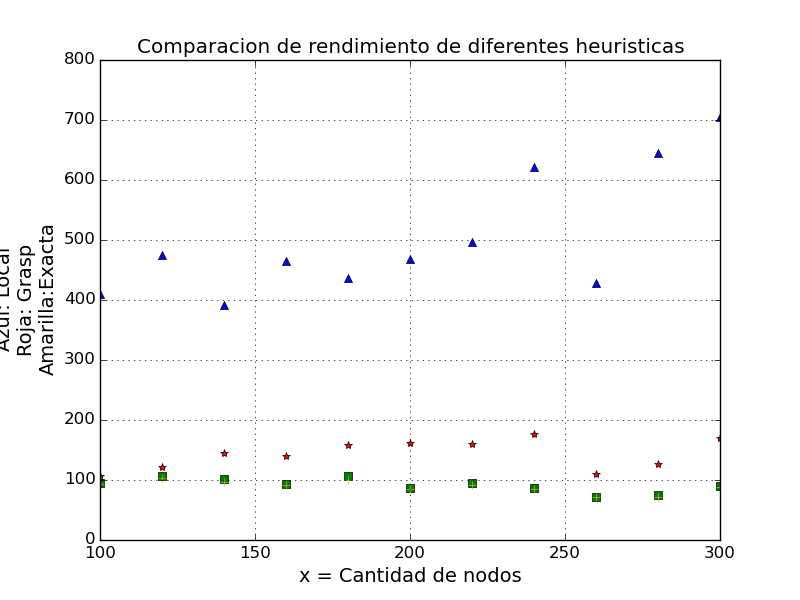
\includegraphics[scale=0.7]{experimentos/performance-optimalidad-intermedios/comparacion_optimalidad.png}
\end{center}

%--------------------------------------------------------------------------------------

\subsubsection{Grafos aleatorios de alta densidad de aristas}
\textbf{Parametros del experimento:}
\begin{itemize}
	\item Parametro Beta GRASP: $\frac{cantNodos}{128}$
	\item Cantidad de grafos analizados: 53
	\item Cantidad minima de nodos: 10
	\item Cantidad maxima de nodos: 280
	\item Rango peso $w_1$: [0..250]
	\item Rango peso $w_2$: [0..400]
	\item Cota de $w_1$: 200
	\item Cantidad minima de aristas: $\frac{n * (n-1)}{3}$
	\item Cantidad maxima de aristas: $\frac{n * (n-1)}{2}$
\end{itemize}

\vspace{1cm}

\textbf{Resultados del analisis (Golosa):}
\begin{lstlisting}[frame=single]	
	Tiempo promedio microsegundos heuristica: 4569.584
	Tiempo promedio microsegundos exacto: 19571.283
	Heuristica da la solucion optima: 83.018% de los casos
	Lejania promedio de la heuristica a la solucion optima: 4.990%
	Desv. estandar de la lejania entre las soluciones: 18.1754
	Minima lejania entre bqlocal y exacta: 0
	Maxima lejania entre bqlocal y exacta: 110.300%
\end{lstlisting}

\textbf{Resultados del analisis (Busqueda local):}
\begin{lstlisting}[frame=single]	
	Tiempo promedio microsegundos heuristica: 550.485
	Tiempo promedio microsegundos exacto: 19571.283
	Heuristica da la solucion optima: 13.207% de los casos
	Lejania promedio de la heuristica a la solucion optima: 1042.275%
	Desv. estandar de la lejania entre las soluciones: 1153.29
	Minima lejania entre bqlocal y exacta: 0
	Maxima lejania entre bqlocal y exacta: 4473.000%
\end{lstlisting}

\textbf{Resultados del analisis (Metaheuristica GRASP):}
\begin{lstlisting}[frame=single]	
	Tiempo promedio microsegundos heuristica: 3637.888
	Tiempo promedio microsegundos exacto: 19571.283
	Heuristica da la solucion optima: 83.018% de los casos
	Lejania promedio de la heuristica a la solucion optima:  3.611%
	Desv. estandar de la lejania entre las soluciones: 12.1007
	Minima lejania entre bqlocal y exacta: 0
	Maxima lejania entre bqlocal y exacta: 73.300%
\end{lstlisting}

\vspace{2cm}

\begin{center}	
	\textbf{Distribucion de los resultados}\\
	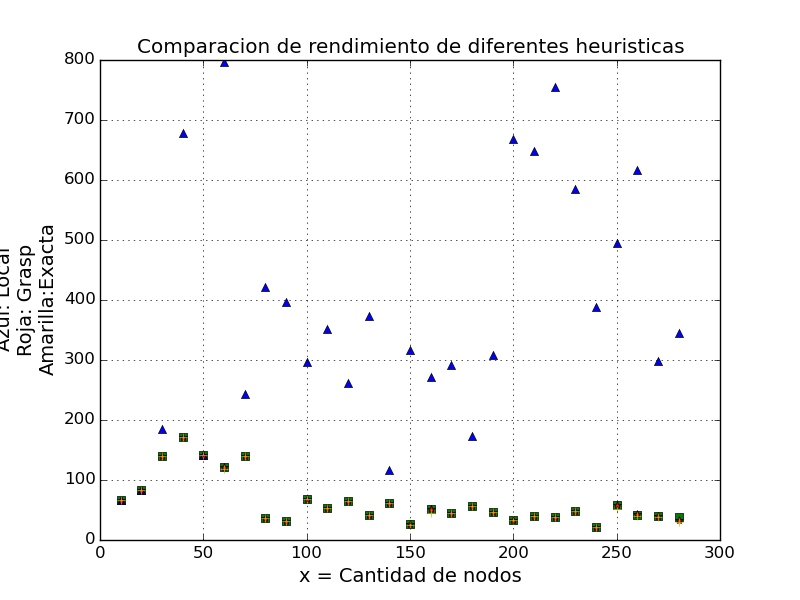
\includegraphics[scale=0.7]{experimentos/performance-optimalidad-cliques_beta_n_over_128/comparacion_optimalidad.png}
\end{center}


\textbf{Conclusion: } Ahora analizaremos como se comportan los algoritmos heuristicos(goloso y busqueda local) respecto a los distintos conjuntos de tests y sus resultados.\\

\vspace{0.75cm}
\textbf{Algoritmo Goloso para grafos de baja densidad:}\\
Vemos que el algoritmo goloso tiene optimalidad cercana al 100\%, aqui dio 98.6\% y en la secci\'on propia del algoritmo goloso dio 100\% cuando se trata de grafos con densidad lineal de aristas, en caso de no dar el optimo, tiene un 0.261\% con una desviacion estandar del 2\% de lejan\'ia respecto a la soluci\'on \'optima. Como contraparte, el tiempo de ejecuci\'on es sutilmente superior al del algoritmo exacto(con 4 podas), seguramente(como se puede apreciar en la secci\'on de rendimiento del algoritmo exacto) para grafos con mayor cantidad de nodos, el tiempo de ejecuci\'on del algoritmo exacto se dispare. Consideramos que el algoritmo goloso es una muy buena opcion si se trata de aproximar soluciones optimas para grafos con densidad lineal con una cantidad de nodos considerablemente alta que produzca que el algoritmo exacto no sea viable.\\

\vspace{0.5cm}

\textbf{Algoritmo Goloso para grafos de densidad intermedia:}\\
Para instancias de grafos con densidades intermedias de aristas, podemos ver como baja levemente el nivel de optimalidad a 86\% de aciertos respecto a la soluci\'on exacta. Tambien se incrementaron a  2.59\% la lejan\'ia promedio y a 9.7\% la desviacion estandar de la lejan\'ia. Sin embargo, sigue siendo una muy buena heur\'istica, porque en este caso si, puede apreciarse que el algoritmo exacto tarda un 250\% mas de tiempo en promedio para llegar a la soluci\'on. Teniendo en cuenta que la cantidad de nodos de los grafos generados va disminuyendo a medidad que aumentamos la densidad(por cuestiones pr\'acticas de realizar los tests en el hardware disponible), observamos que para densidades mas altas de aristas en los grafos testeados empieza a ser una muy buena alternativa la soluci\'on golosa, siempre y cuando el contexto de aplicaci\'on acepte los estimadores de lejan\'ia al optimo.

\vspace{0.5cm}

\textbf{Algoritmo Goloso para grafos de alta densidad:}\\
Finalmente, para el caso mas complicado para el algoritmo exacto(recordemos que en la complejidad, el grado de los nodos es la cantidad de llamadas recursivas que realiza y si la densidad es alta el grado promedio va a ser alto dada la distribucion uniforme de las aristas sobre el grafo), la soluci\'on golosa disminuye muy levemente la efectividad con respecto al caso anterior, tiene un 83\% de aciertos a la soluci\'on \'optima, asimismo aumentan los estimadores de lejan\'ia, en promedio a un 4.99\% con una desviaci\'on de 18.17\%. Respecto al tiempo de ejecuci\'on, el algoritmo exacto tarda en promedio 4.28 veces mas de tiempo para obtener la soluci\'on exacta. Para ser el caso mas dificil de los casos de prueba que consideramos, pensamos que los resultados son muy buenos para las aplicaciones pr\'acticas.

\vspace{0.5cm}

\textbf{Algoritmo de Busqueda local para grafos de baja densidad:}\\
Respecto a la heuristica de busqueda local, observamos un 30\% de efectividad, con una lejan\'ia promedio de 87.62\% y una desv. estandar en la lejan\'ia al optimo de 118.5\%, consideramos que 30\% es un numero muy bajo y junto a los indicadores de lejan\'ia, si nos interesa realmente una solucion cercana a la \'optima no elegiriamos esta heur\'istica(al menos no con dijkstra sobre $w_1$ como soluci\'on inicial. Ver Experimentacion de la solucion inicial en la secci\'on busqueda local). Como contraparte, toma aproximadamente la mitad de tiempo que el algoritmo exacto(recordemos que la medicion es por iteracion y para grafos lineales hay 1 iteracion promedio.), no consideramos que sea un buen tradeoff, la mitad del tiempo de ejecuci\'on para esta calidad de soluciones.\\

\vspace{0.5cm}

\textbf{Algoritmo de Busqueda local para grafos de densidad intermedia:}\\
A medida que vamos aumentando la densidad de los grafos, la b\'usqueda local deber\'ia poder mejorar mas la soluci\'on, de hecho cuando analizamos la variaci\'on de la soluci\'on a medida que avanzan las iteraciones, el mejor caso era donde la densidad era m\'axima, lo que atribuiamos a una vecindad de mayor cardinal, pero cuando comparamos optimalidad promedio de la heur\'istica, nos da un numero baj\'isimo, 10\% de aciertos a la soluci\'on optima, con un promedio y dispersi\'on de lejan\'ia enormes. Atribuimos este bajo rendimiento a la soluci\'on inicial provista realizando dijkstra sobre $w_1$, mas adelante cuando analicemos GRASP, para ciertos valores del par\'ametro beta(bajos, para que se acerque la soluci\'on randomizada a la heur\'istica golosa pura), los experimentos representar\'an una b\'usqueda local alimentada inicialmente por un algoritmo de mayor optimalidad. Dado que la cantidad promedio de iteraciones para densidades intermedias nos dio cercano a 4 iteraciones, el tiempo de ejecuci\'on(por iteracion) multiplicado por 4, nos da como resultado que el algoritmo de b\'usqueda local tarda un tercio del tiempo que el algoritmo exacto, nuevamente, no consideramos que sea un tradeoff aceptable dada la calidad de las soluciones.

\vspace{0.5cm}

\textbf{Algoritmo de Busqueda local para grafos de alta densidad:}\\
Este caso es casi id\'entico al anterior con respecto a la optimalidad de las soluciones, tal vez un poco peor, pero despreciable, lo \'unico que vari\'o considerablemente fue el tiempo de ejecucion del algoritmo exacto a 19571 microsegundos y la cantidad de iteraciones promedio de la b\'usqueda local a 5 iteraciones promedio con un tiempo por iteracion de 550 microsegundos. Veamos entonces que el algoritmo de b\'usqueda local se ejecuta aproximadamente 7 veces mas rapido que el algoritmo exacto. Las conclusiones son las mismas que en el caso de densidad intermedia, no consideramos que sea un buen tradeoff dado el \texttt{baj\'isimo} numero de aciertos a la soluci\'on optima y la enorme lejan\'ia al optimo.

\vspace{0.5cm}

Como conclusi\'on de b\'usqueda local consideramos que depende mucho de la soluci\'on inicial la calidad final de las soluciones obtenidas(nuevamente, ver seccion de variacion de soluciones iniciales en seccion busqueda local). Utilizar\'iamos un esquema de b\'usqueda local para refinar soluciones relativamente buenas obtenidas con algun otro m\'etodo inicial.

\vspace{0.5cm}

\textbf{Algoritmo de Metaheuristica GRASP para grafos de baja densidad:}\\
Notamos como primer observacion que la metaheuristica toma mas tiempo que el algoritmo exacto, y al tener un 57\% de porcentaje de aciertos con respecto a la soluci\'on \'optima, descartamos que sea una buena heur\'istica para este tipo de grafos, sin importar la lejania ni la dispersion de la lejan\'ia, en menos tiempo podemos obtener la solucion exacta.

\vspace{0.5cm}

\textbf{Algoritmo de Metaheuristica GRASP para grafos de densidad intermedia:}\\
Observamos que la heuristica no es muy efectiva, con una alta lejania y dispersion de lejania respecto a la solucion optima, a pesar de que el tiempo que toma sea la mitad que el algoritmo exacto, no lo utilizariamos como heuristica para este tipo de grafos.

\vspace{0.5cm}

\textbf{Algoritmo de Metaheuristica GRASP para grafos de alta densidad:}\\
Notemos que toma menos tiempo que el algoritmo goloso(y mucho menos tiempo que el algoritmo exacto), nos provee el mismo alto porcentaje de efectividad respecto a la solucion optima que el algoritmo goloso, y aun mejor, la lejan\'ia promedio y dispersion de esta, se disminuyeron respecto a la soluci\'on. Para este tipo de grafos, con alta densidad, encontramos que con este parametro beta, ocurrian este tipo de mejoras, si bien esto es el resultado de una muestra de toda la familia de grafos de alta densidad, podriamos considerar aplicar esta heuristica aun mas que la heuristica golosa para resolver el problema de manera aproximada.
\vspace{0.5cm}

\subsubsection{Gr\'aficos de distribucion de las soluciones}
\vspace{0.5cm}
\textbf{Distribuci\'on de soluciones para grafos de alta densidad:}\\
Podemos observar que las soluci\'ones de b\'usqueda local siempre estan lejos del \'optimo indicado por un + amarillo en el eje Y. Con respecto a GRASP, algoritmo goloso y algoritmo exacto se encuentran casi superpuestos, salvo casos particulares.

\vspace{0.5cm}
\textbf{Distribuci\'on de soluciones para grafos de densidad intermedia:}\\
Se observa que los valores de las soluciones provistos por busqueda local estan sutilmente mas cerca de los demas algoritmos, igual siguen estando relativamente lejos, respecto a las otras heuristicas(Golosa y GRASP) comienzan a verse su "despegue" de la soluci\'on \'optima, mas que nada en la metaheuristica GRASP.

\vspace{0.5cm}
\textbf{Distribuci\'on de soluciones para grafos de baja densidad:}\\
Finalmente aqui observamos que la soluci\'on de busqueda local sigue "lejos" del \'optimo. Asimismo, GRASP tampoco provee la soluci\'on \'optima ni una \texttt{muy cercana}, como si lo hace la heur\'istica golosa con su casi perfecto indice de aciertos respecto al algoritmo exacto.

\subsection{Experimentacion pura entre heuristicas}
En esta secci\'on experimentaremos para varios conjuntos aleatorios de grafos de diferentes densidades con las heur\'isticas implementadas,sin tener en cuenta la soluci\'on exacta, para poder realizar experimentos con una mayor cantidad de nodos y aristas en las instancias. Dados los resultados, analizaremos de las 3 heur\'isticas implementadas cual obtiene las soluciones con peso $w_2$ menor, y de esta forma, mas cercanas a la solucion optima(que siempre es menor o igual al minimo de las 3 heuristicas, por definicion de solucion optima).\\

Esto se realizara, para cada ejecucion de las 3 heuristicas, incrementando un contador en la que corresponda si su peso $w_2$ es minimo, al final tendremos, para cada heuristica, cuantas veces dio la minima solucion, y la cantidad total de instancias testeadas, con estos datos podremos realizar los analisis estadisticos.

\subsubsection{Grafos aleatorios de alta densidad de aristas}
\textbf{Parametros del experimento:}
\begin{itemize}
	\item Parametro Beta GRASP: $\frac{cantNodos}{128}$
	\item Cantidad de grafos analizados: 17
	\item Cantidad minima de nodos: 10
	\item Cantidad maxima de nodos: 340
	\item Rango peso $w_1$: [0..250]
	\item Rango peso $w_2$: [0..400]
	\item Cota de $w_1$: 200
	\item Cantidad minima de aristas: $\frac{n * (n-1)}{3}$
	\item Cantidad maxima de aristas: $\frac{n * (n-1)}{2}$
\end{itemize}

\textbf{Resultados del analisis:}
\begin{lstlisting}[frame=single]	
	Porcentaje de instancias donde da el minimo w2:
        Golosa: 94.1%
        Busqueda local: 17.6%
        Grasp: 41.1%
\end{lstlisting}


\subsubsection{Grafos aleatorios de densidad intermedia de aristas}
\textbf{Parametros del experimento:}
\begin{itemize}
	\item Parametro Beta GRASP: $\frac{cantNodos}{128}$
	\item Cantidad de grafos analizados: 226
	\item Cantidad minima de nodos: 100
	\item Cantidad maxima de nodos: 600
	\item Rango peso $w_1$: [0..250]
	\item Rango peso $w_2$: [0..400]
	\item Cota de $w_1$: 200
	\item Cantidad minima de aristas: $ n * \sqrt n$
	\item Cantidad maxima de aristas: $ 5 * n * \sqrt n$
\end{itemize}

\textbf{Resultados del analisis:}
\begin{lstlisting}[frame=single]	
	Cantidad de instancias donde da el minimo w2:
        Golosa: 96.9%
        Busqueda local: 6.6%
        Grasp: 33.1%
\end{lstlisting}

%partes relevantes del codigo
\section{Ap\'endice: C\'odigo fuente relevante}


\subsection{Algoritmo exacto para la resolucion de CACM}
\lstinputlisting[language=C++,tabsize=4, numbers=left, numberstyle=\tiny\color{black},mathescape=true, backgroundcolor=\color{gray}, rulecolor=\color{black}, keywordstyle=\color{blue}, commentstyle=\color{dkgreen},stringstyle=\color{mauve}, numbersep=5pt, basicstyle=\scriptsize]{codigo/exacto.cpp}

\subsection{Heuristicas constructivas golosas I: En cada paso tomar el minimo f2 dentro de las soluciones factibles(con f1 acotada)}
\lstinputlisting[language=C++,tabsize=4, numbers=left, numberstyle=\tiny\color{black},mathescape=true, backgroundcolor=\color{gray}, rulecolor=\color{black}, keywordstyle=\color{blue}, commentstyle=\color{dkgreen},stringstyle=\color{mauve}, numbersep=5pt, basicstyle=\scriptsize]{codigo/golosa1.cpp}

\subsection{Heuristicas constructivas golosas II: En cada paso tomar el minimo cociente de f1/f2 dentro de las soluciones factibles(con f1 acotada)}
\lstinputlisting[language=C++,tabsize=4, numbers=left, numberstyle=\tiny\color{black},mathescape=true, backgroundcolor=\color{gray}, rulecolor=\color{black}, keywordstyle=\color{blue}, commentstyle=\color{dkgreen},stringstyle=\color{mauve}, numbersep=5pt, basicstyle=\scriptsize]{codigo/golosa2.cpp}

\subsection{Heuristicas de busqueda local}
\lstinputlisting[language=C++,tabsize=4, numbers=left, numberstyle=\tiny\color{black},mathescape=true, backgroundcolor=\color{gray}, rulecolor=\color{black}, keywordstyle=\color{blue}, commentstyle=\color{dkgreen},stringstyle=\color{mauve}, numbersep=5pt, basicstyle=\scriptsize]{codigo/busquedalocal.cpp}

\subsection{Metaheuristica GRASP: Solucion propuesta}
\lstinputlisting[language=C++,tabsize=4, numbers=left, numberstyle=\tiny\color{black},mathescape=true, backgroundcolor=\color{gray}, rulecolor=\color{black}, keywordstyle=\color{blue}, commentstyle=\color{dkgreen},stringstyle=\color{mauve}, numbersep=5pt, basicstyle=\scriptsize]{codigo/grasp.cpp}


%info acerca del entregable de este trabajo
\section{Ap\'endice: Entregable e instrucciones de compilacion y benchmarking}
\subsection{Estructura de directorios}
%\begin{itemize}
%	\item \textbf{ej1:} Contiene el codigo fuente en java del ejercicio 1, tanto como los scripts de compilacion nativa, testeo y graficacion, casos de tests, mediciones, y graficos.
%	\item \textbf{ej2:} Contiene el codigo fuente en C++ del ejercicio 2 y su Makefile para compilar.
%	\item \textbf{ej3:} Contiene el codigo fuente en java del ejercicio 3, tanto como los scripts de compilacion nativa, testeo y graficacion, casos de tests, mediciones y graficos.
	%\item \textbf{informe:} Contiene los fuentes de latex, imagenes y codigo relevante junto al pdf del informe 
	%\item \textbf{casos:}	Contiene el programa que genera los casos del ej2
%\end{itemize}

\subsection{Compilacion y ejecucion}
%\begin{itemize}
	%\item \textbf{ej1:} Ejecutando ./compilacionNativa.sh se compila el programa, se crean y resuelven tests aleatorios tomando tiempos y se grafican en png los resultados.
	%\item \textbf{ej2:} utilizando el Makefile y corriendo el ejecutable.
	%\item \textbf{ej3:} Ejecutando ./compilacionNativa.sh se compila el programa, se crean y resuelven tests aleatorios tomando tiempos y se grafican en png los resultados.
%\end{itemize}

\subsection{Benchmarking}
%\begin{itemize}
	%\item \textbf{ej1:} pasandole el parametro --take-time $<$cant\_repeticiones$>$ se repite la ejecucion cant\_repeticiones veces tomando tiempo promedio en microsegundos . --generate-tests $<$cards number$>$ $<$randMin$>$ $<$randMax$>$ genera casos aleatorios correspondientes y los arroja por stdout.
	%\item \textbf{ej2:} Utilizando el programa especifico en la carpeta casos.
	%\item \textbf{ej1:} pasandole el parametro --take-time $<$cant\_repeticiones$>$ se repite la ejecucion cant\_repeticiones veces tomando tiempo promedio en microsegundos . --generate-tests $<$dimension$>$ $<$powerUp inicial$>$ genera casos aleatorios correspondientes y los arroja por stdout.y graficos.
%\end{itemize}

\end{document}

